\documentclass[a4paper]{article}
\usepackage[left=2cm, right=2cm,bottom=2cm]{geometry}
\usepackage{lipsum}
\usepackage{tikzpagenodes}
\usepackage{pgfplots}
\usepackage{tikz}
\usepackage{tikz-3dplot}
\usetikzlibrary{arrows,decorations.pathmorphing,backgrounds,positioning,fit,matrix}
\pgfplotsset{compat=1.8}
\usepackage{graphics} % for pdf, bitmapped graphics files
\usepackage{graphicx}%<----remove demo in your file
\usepackage{epsfig} % for postscript graphics files
\usepackage[colorlinks=true,citecolor=green]{hyperref}
\usepackage{cite}
\usepackage{amsmath,amssymb,amsfonts}
\usepackage{algorithmic}
\usepackage{graphicx}
\usepackage{url}
\usepackage{cite}
\usepackage{bm}
\usepackage{pbox}
\usepackage{siunitx,booktabs,etoolbox}
\usepackage{ulem}
\usepackage{titling}
\usepackage{float}
%\usepackage{pgf,tikz,pgfplots}
%\pgfplotsset{compat=1.15}
%\usepackage{mathrsfs}

\usetikzlibrary{arrows}

\def\BibTeX{{\rm B\kern-.05em{\sc i\kern-.025em b}\kern-.08em
		T\kern-.1667em\lower.7ex\hbox{E}\kern-.125emX}}
\title{Ex3: MRF, Deformable Models \& Geometric Priors}
\author{Xiao Hu, emails: \url{xiahaa@space.dtu.dk}}
\begin{document}
	\maketitle
	\thispagestyle{empty}
	\section{Feed Forward Neural Network}
	Neural network used in this exercise is shown in Figure~\ref{fig1}:
	\begin{figure*}[thtbp]
	\setlength{\fboxrule}{0.0pt}      
	\framebox{\parbox{6.5in}{
			\centering
			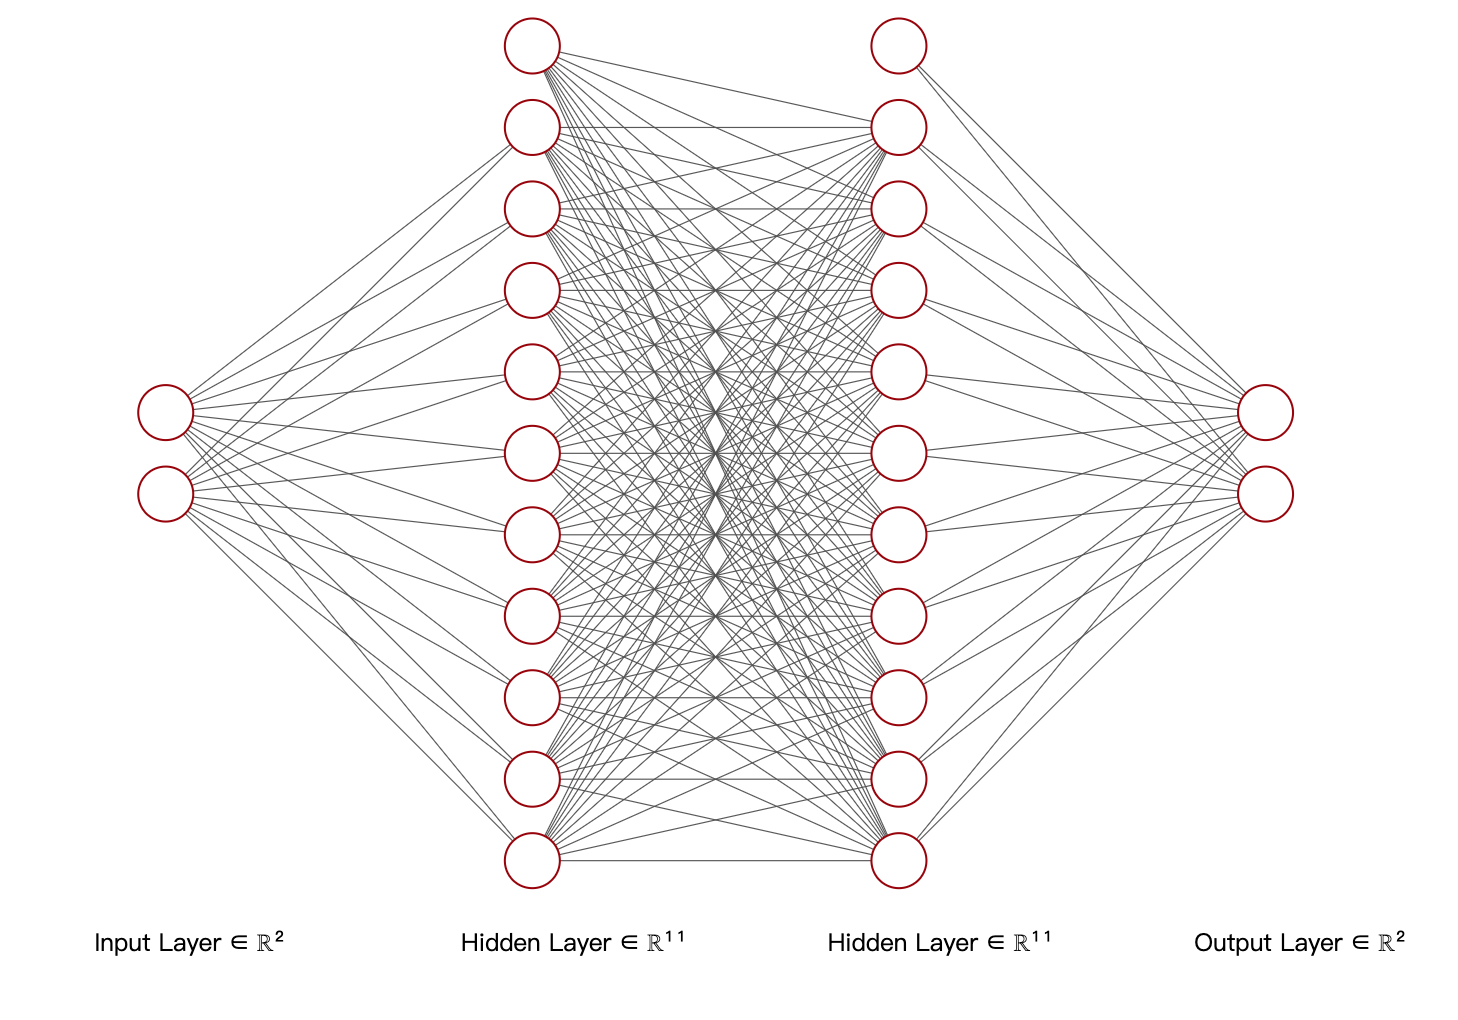
\includegraphics[scale=0.4]{figures/nn1.png}
	}} 
	\label{fig1}
	\caption{$3$ layers neural network used in the first exercise.}
\end{figure*}
	\begin{figure*}[thtbp]
	\setlength{\fboxrule}{0.0pt}      
	\framebox{\parbox{6.5in}{
	\centering
	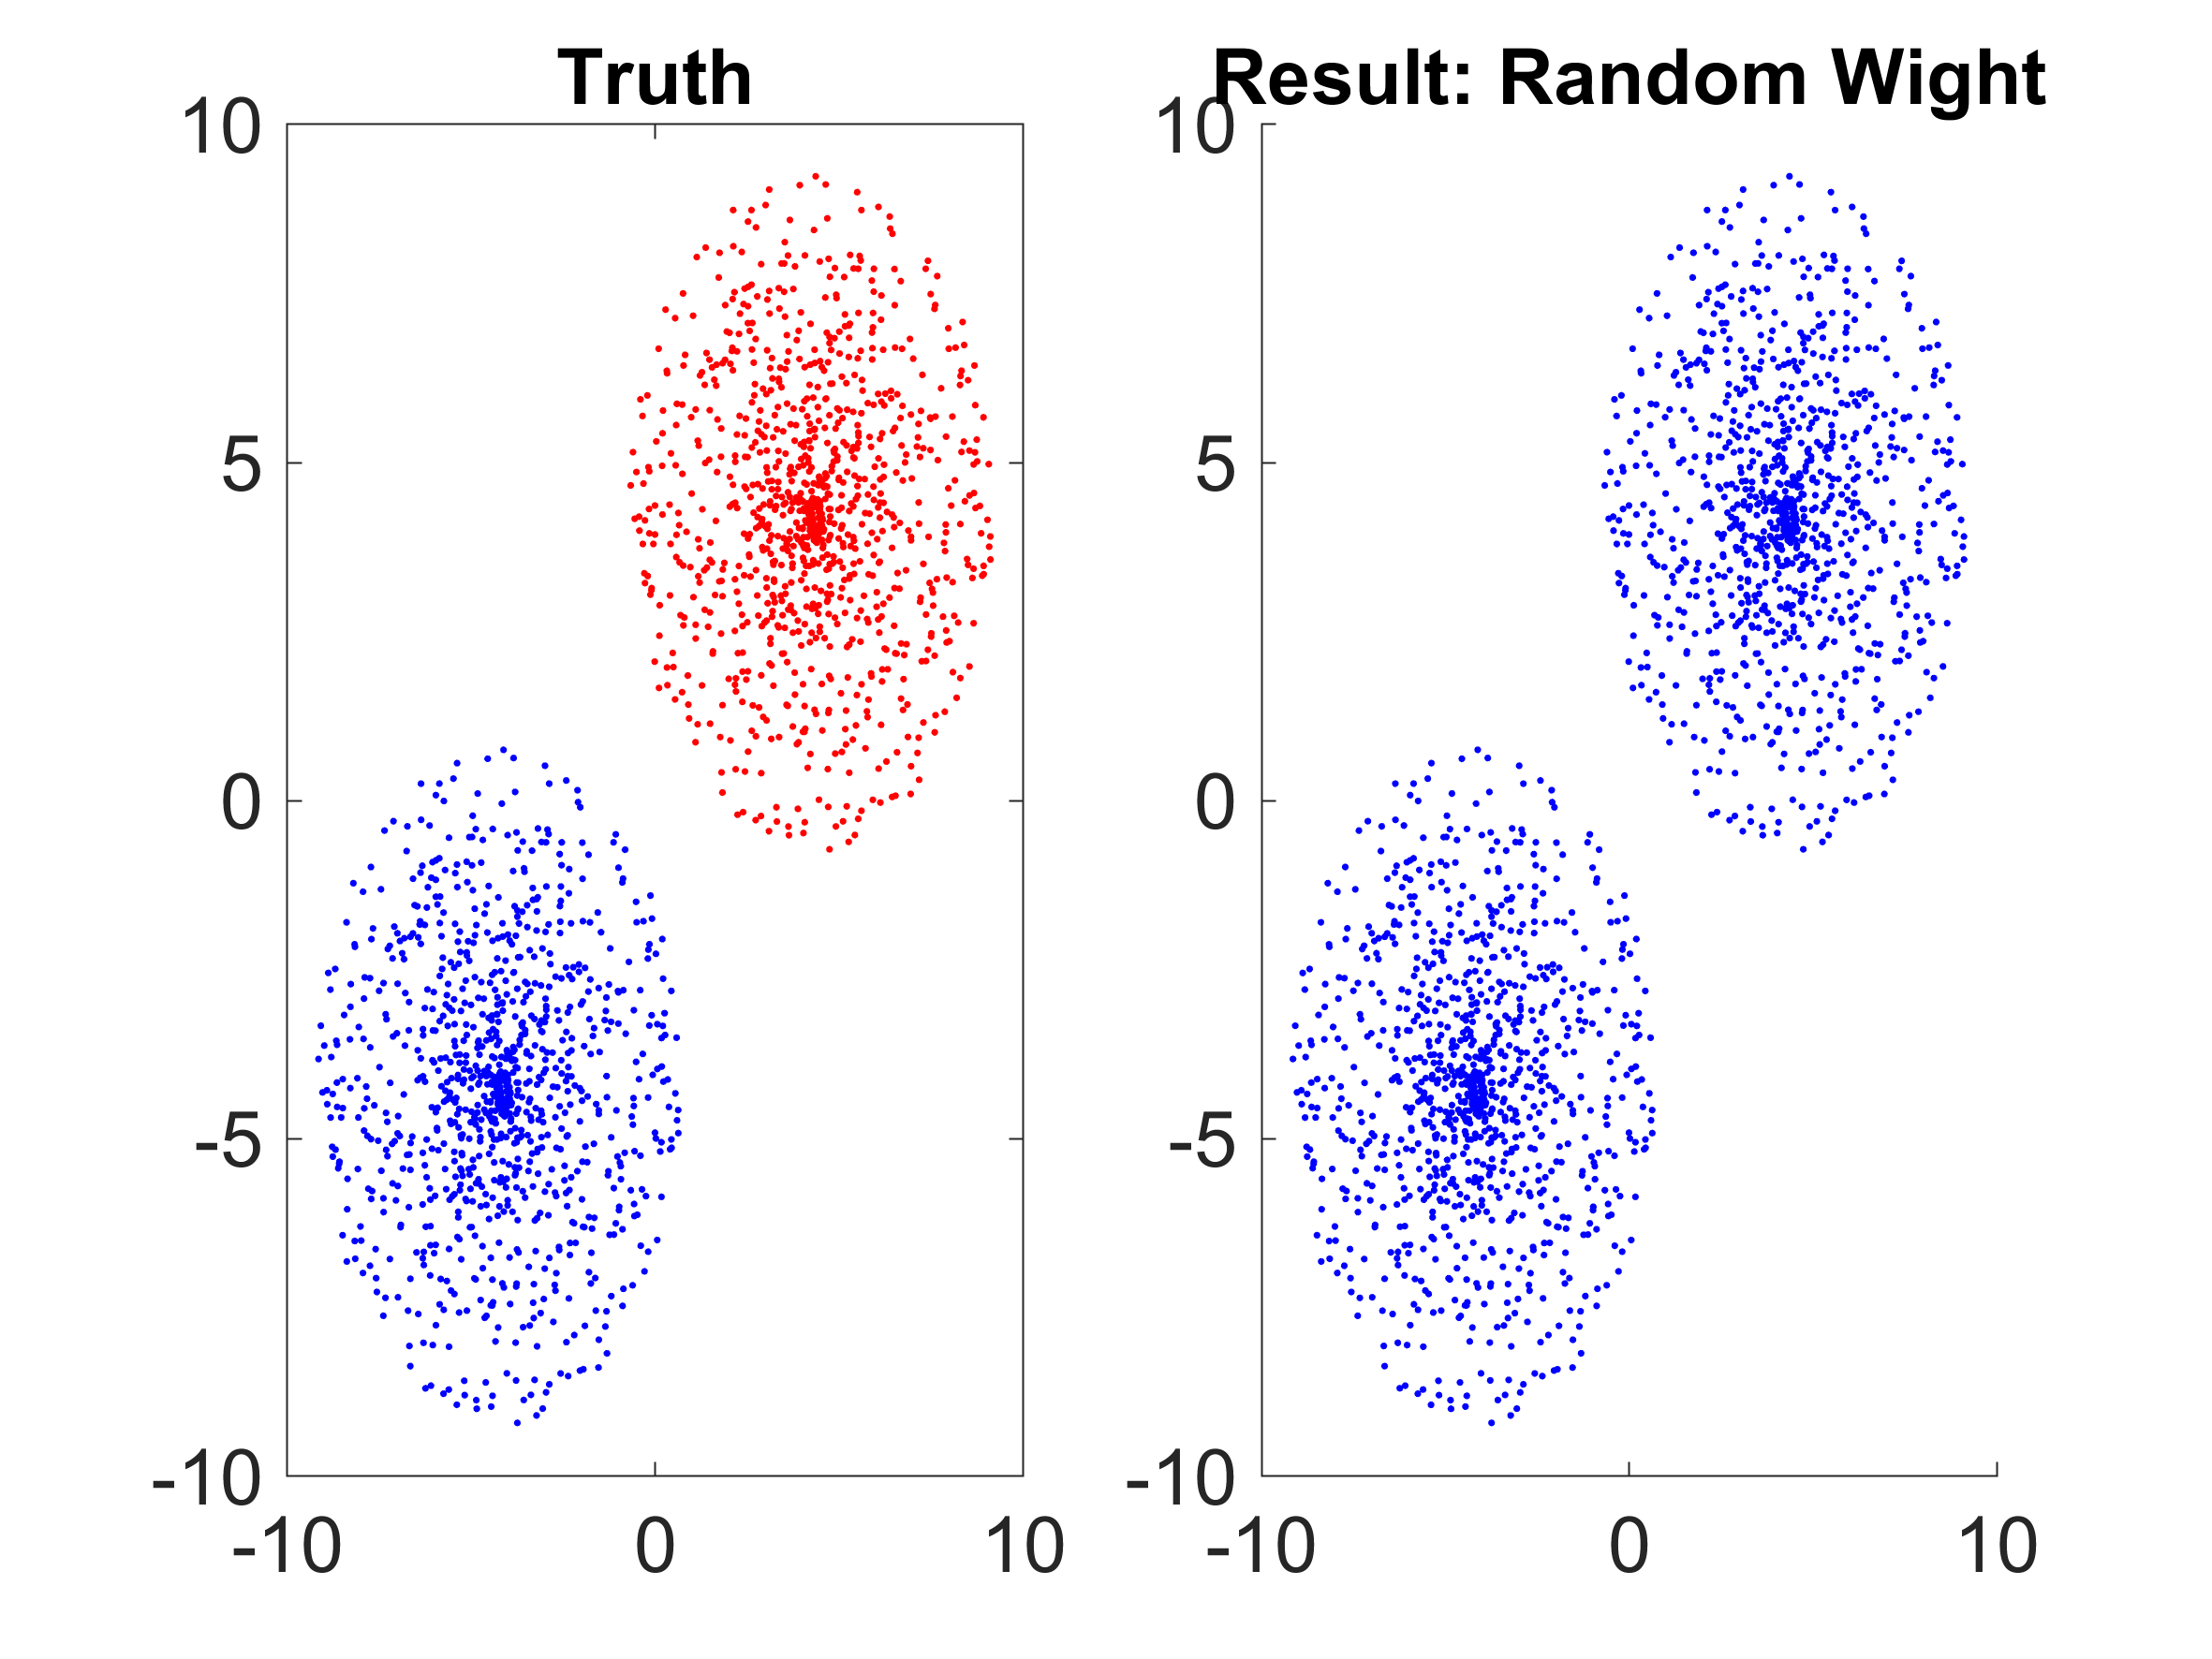
\includegraphics[scale=0.4]{figures/ex2_1.png}
	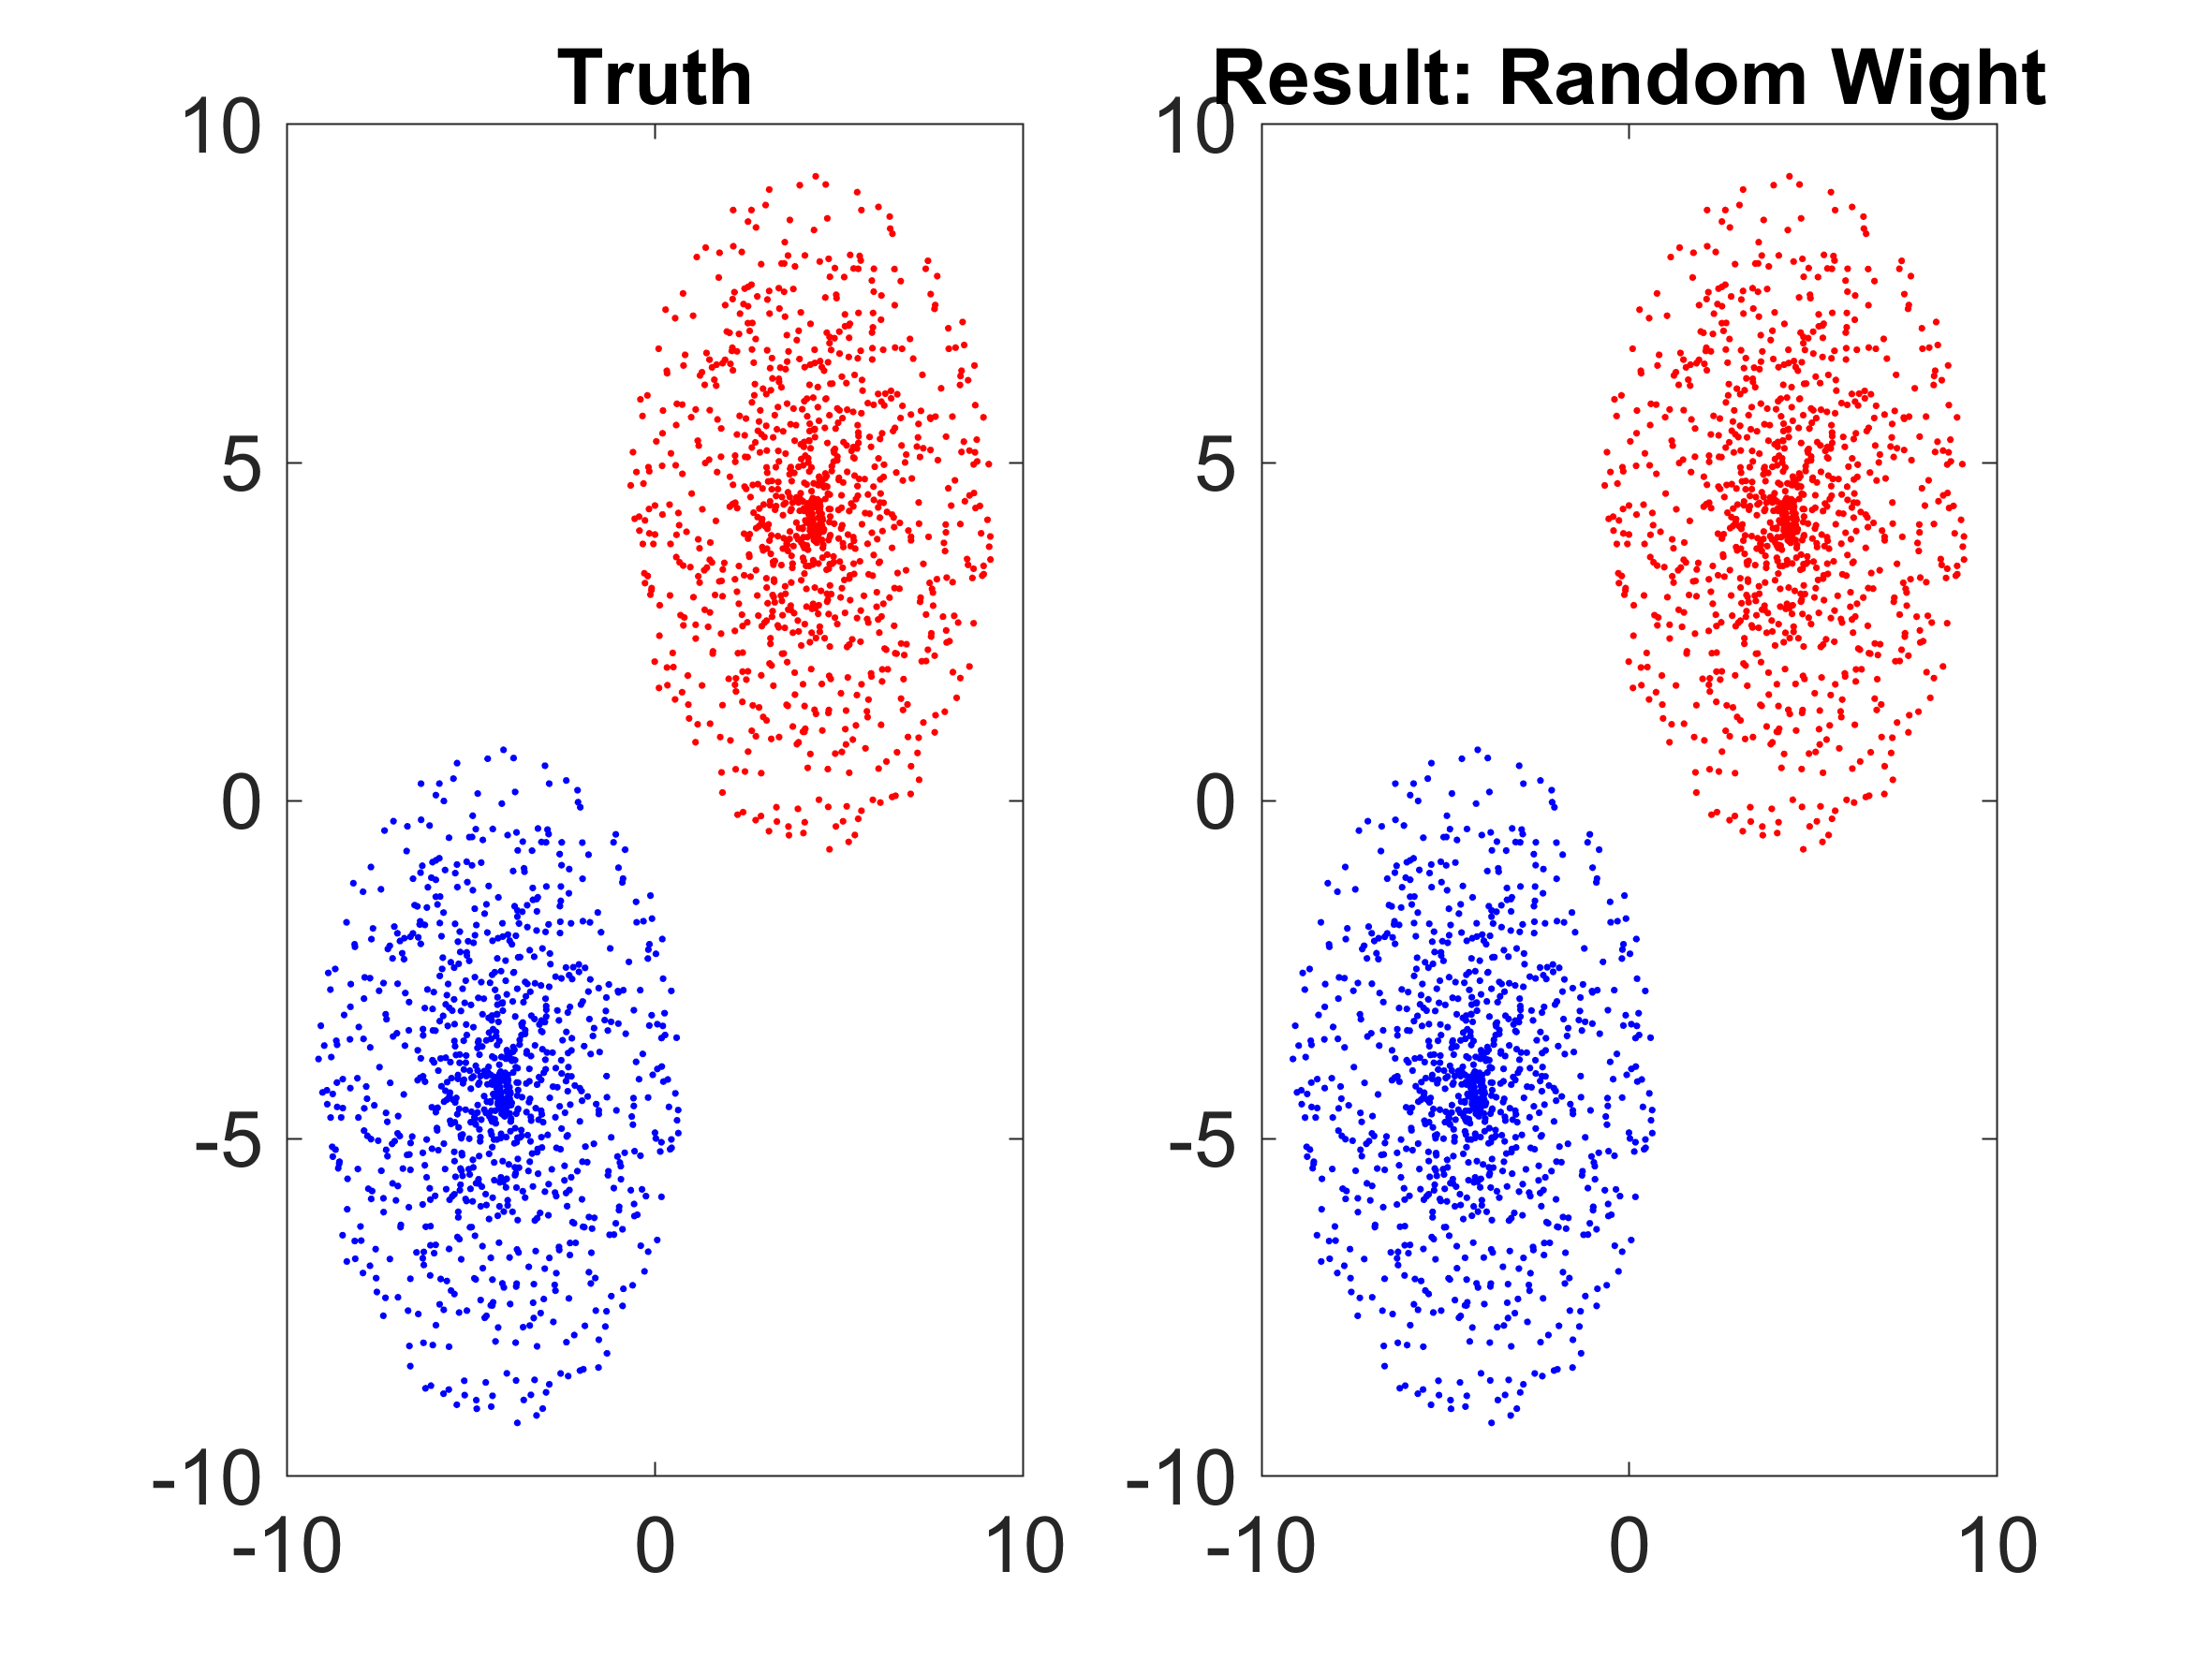
\includegraphics[scale=0.4]{figures/ex2_2.png}
	}} 
    \caption{Point cloud segmentation results: left image shows the segmentation result after initialization using random wieghts, while right image shows the final segmentation result.}
\end{figure*}
  \begin{figure*}[thpb]
	\setlength{\fboxrule}{0.0pt}      
	\framebox{\parbox{6.5in}{
			\centering
			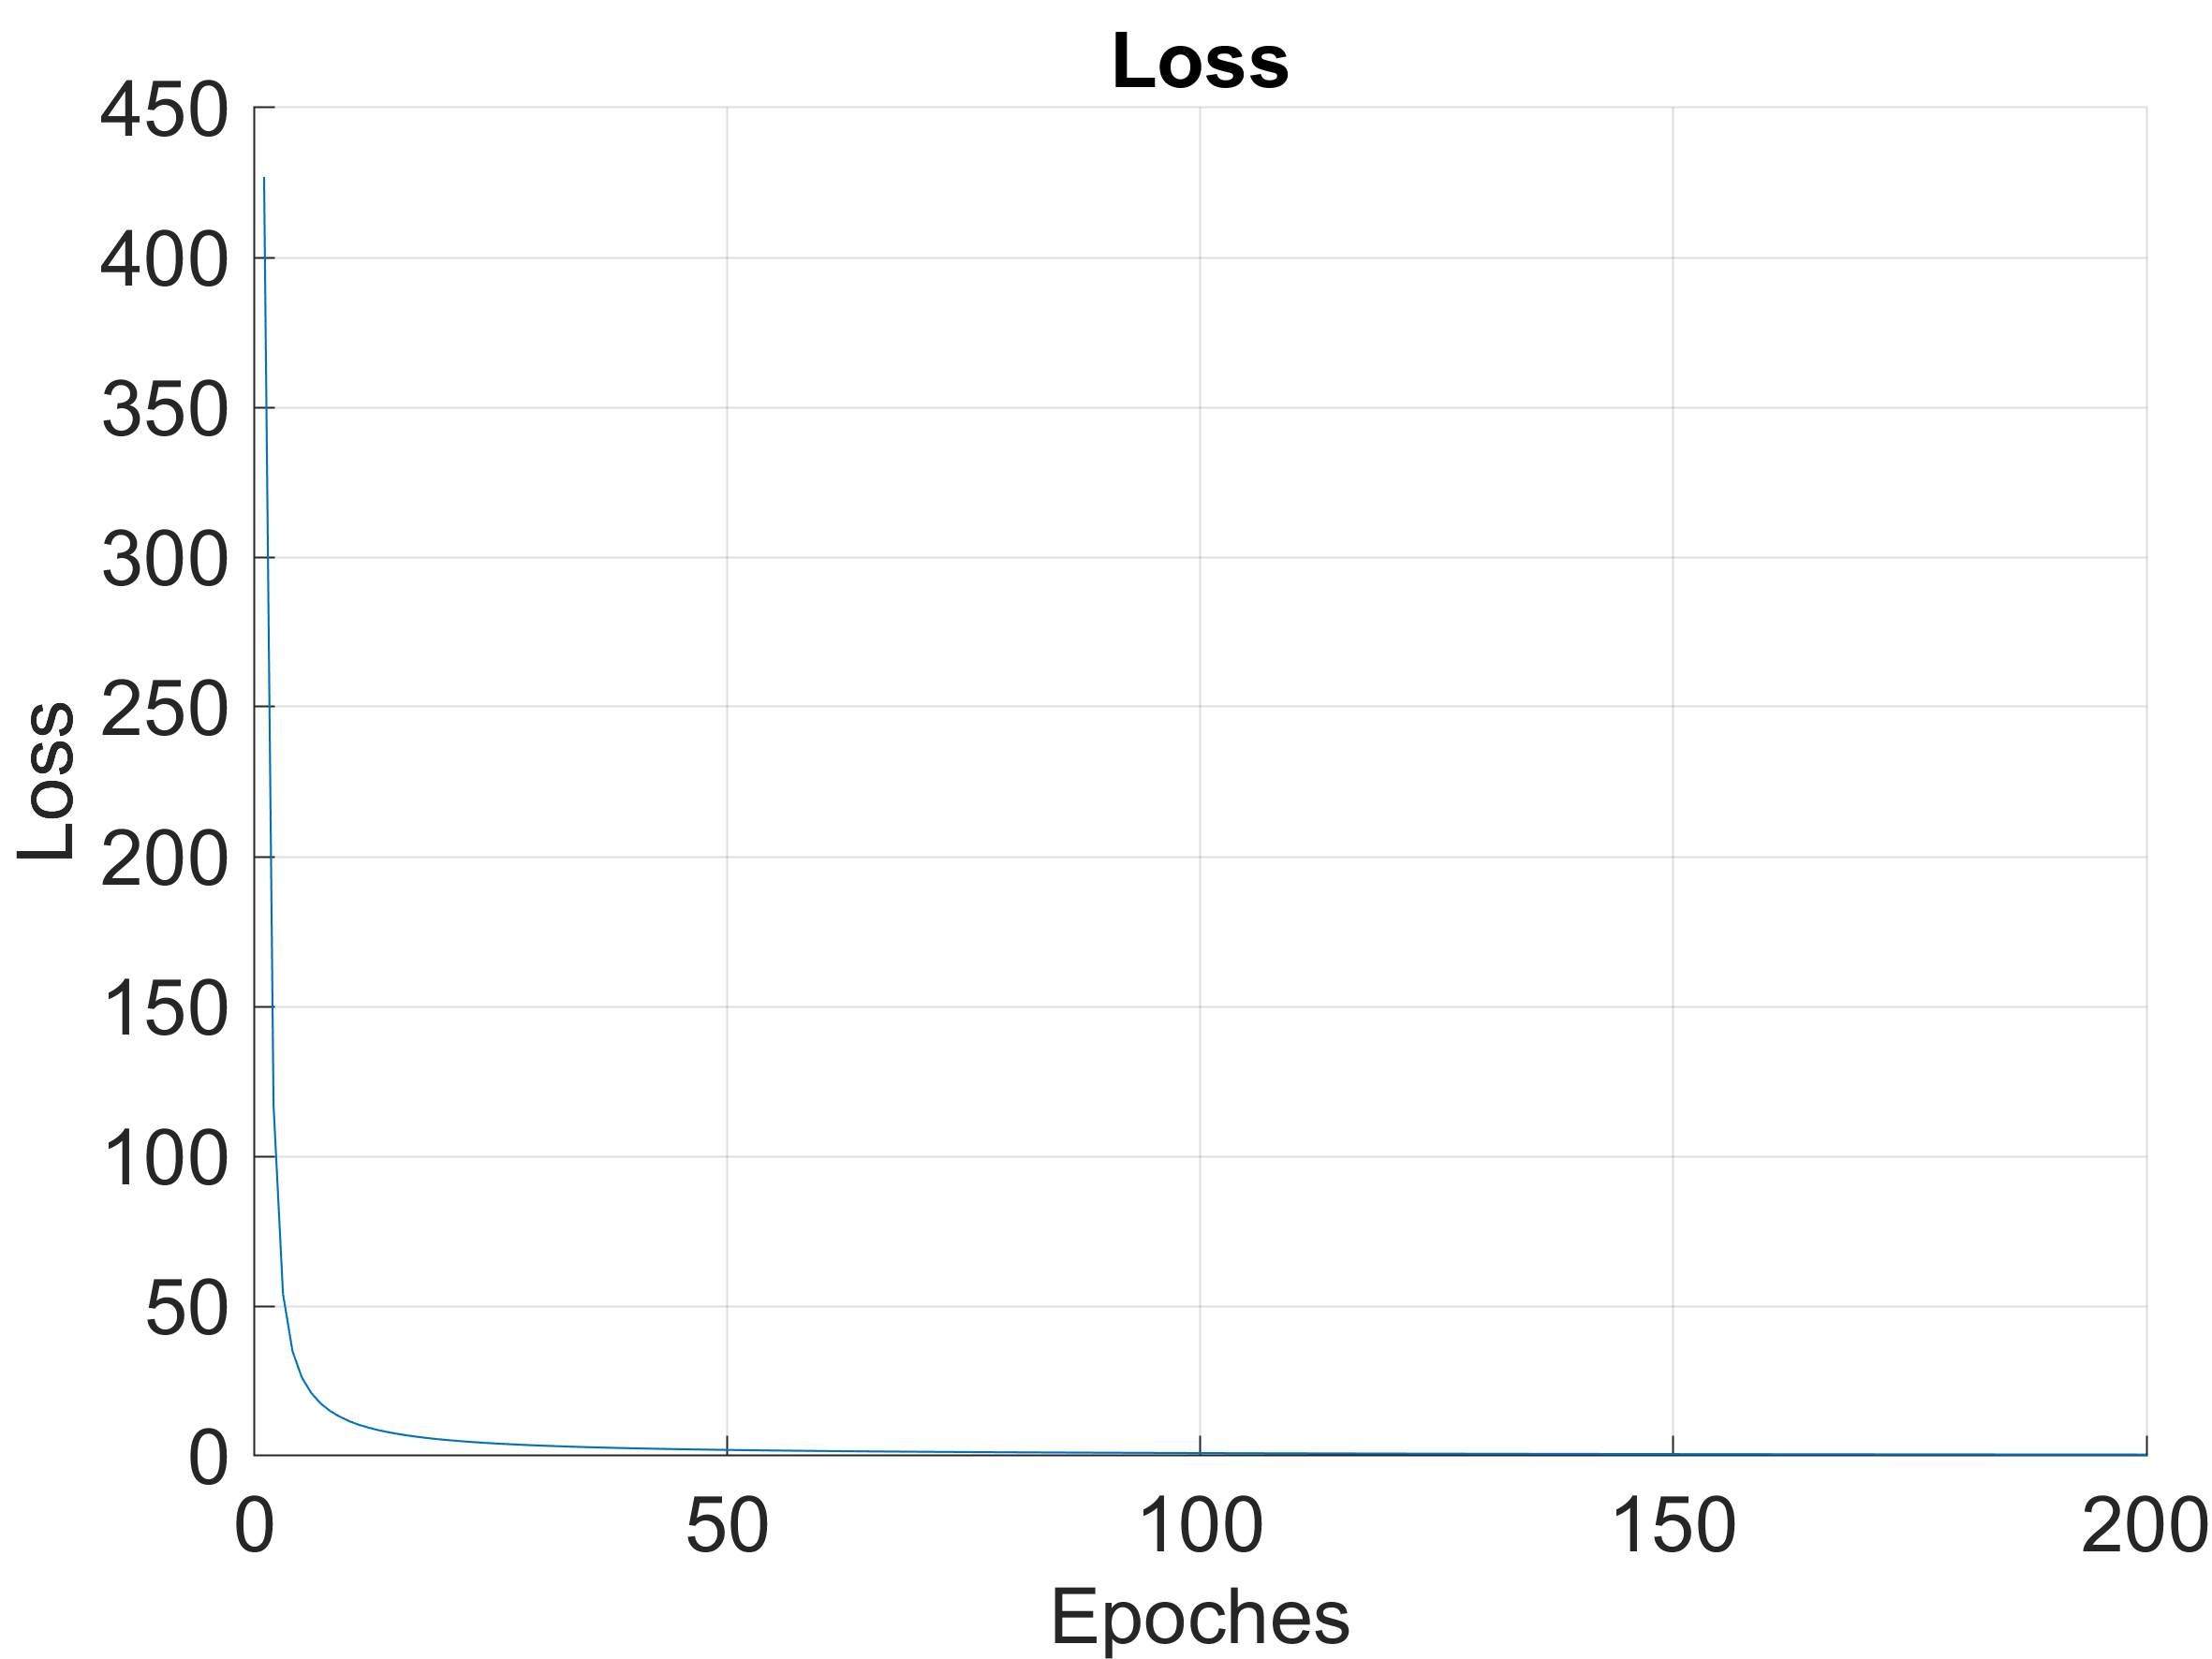
\includegraphics[scale=0.4]{figures/ex2_3.png}
			\hspace{10mm}
			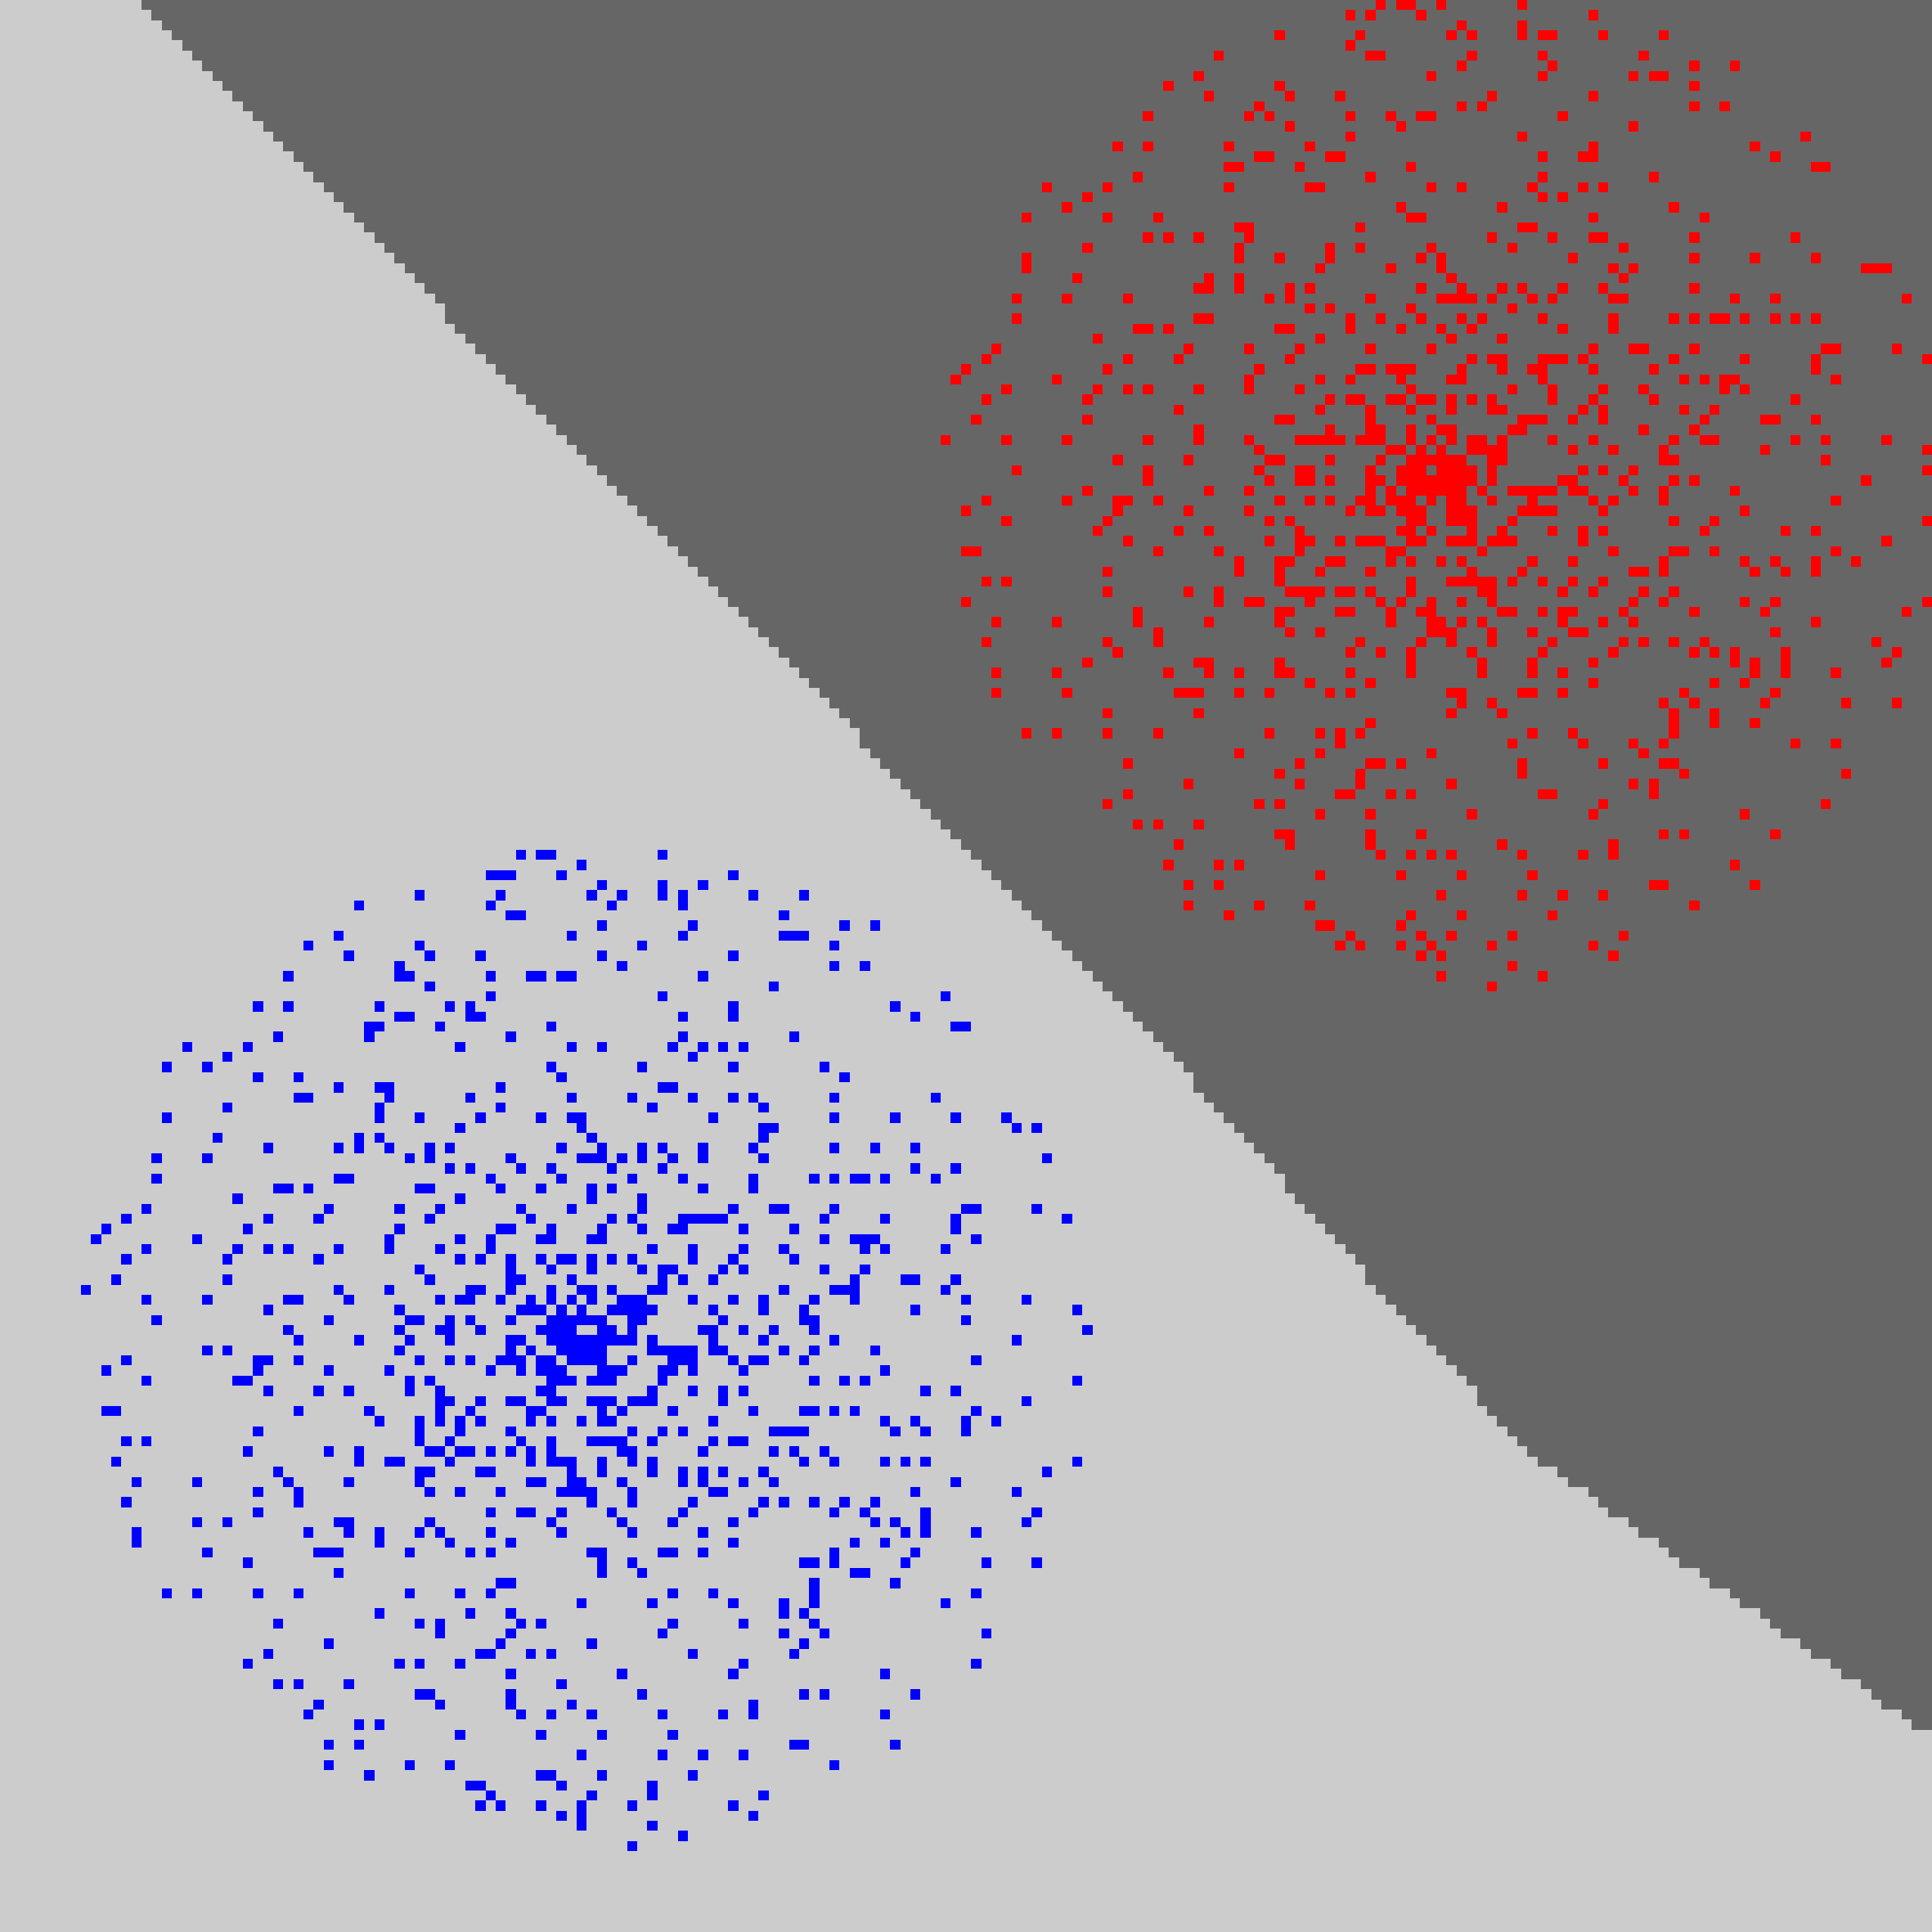
\includegraphics[scale=0.3]{figures/ex2_4.png}
	}} 
	\caption{Left image shows the training loss variations with epochs. Right image shows the segmentation boundary.}
\end{figure*}
	\begin{figure*}[thtbp]
	\setlength{\fboxrule}{0.0pt}      
	\framebox{\parbox{6.5in}{
			\centering
			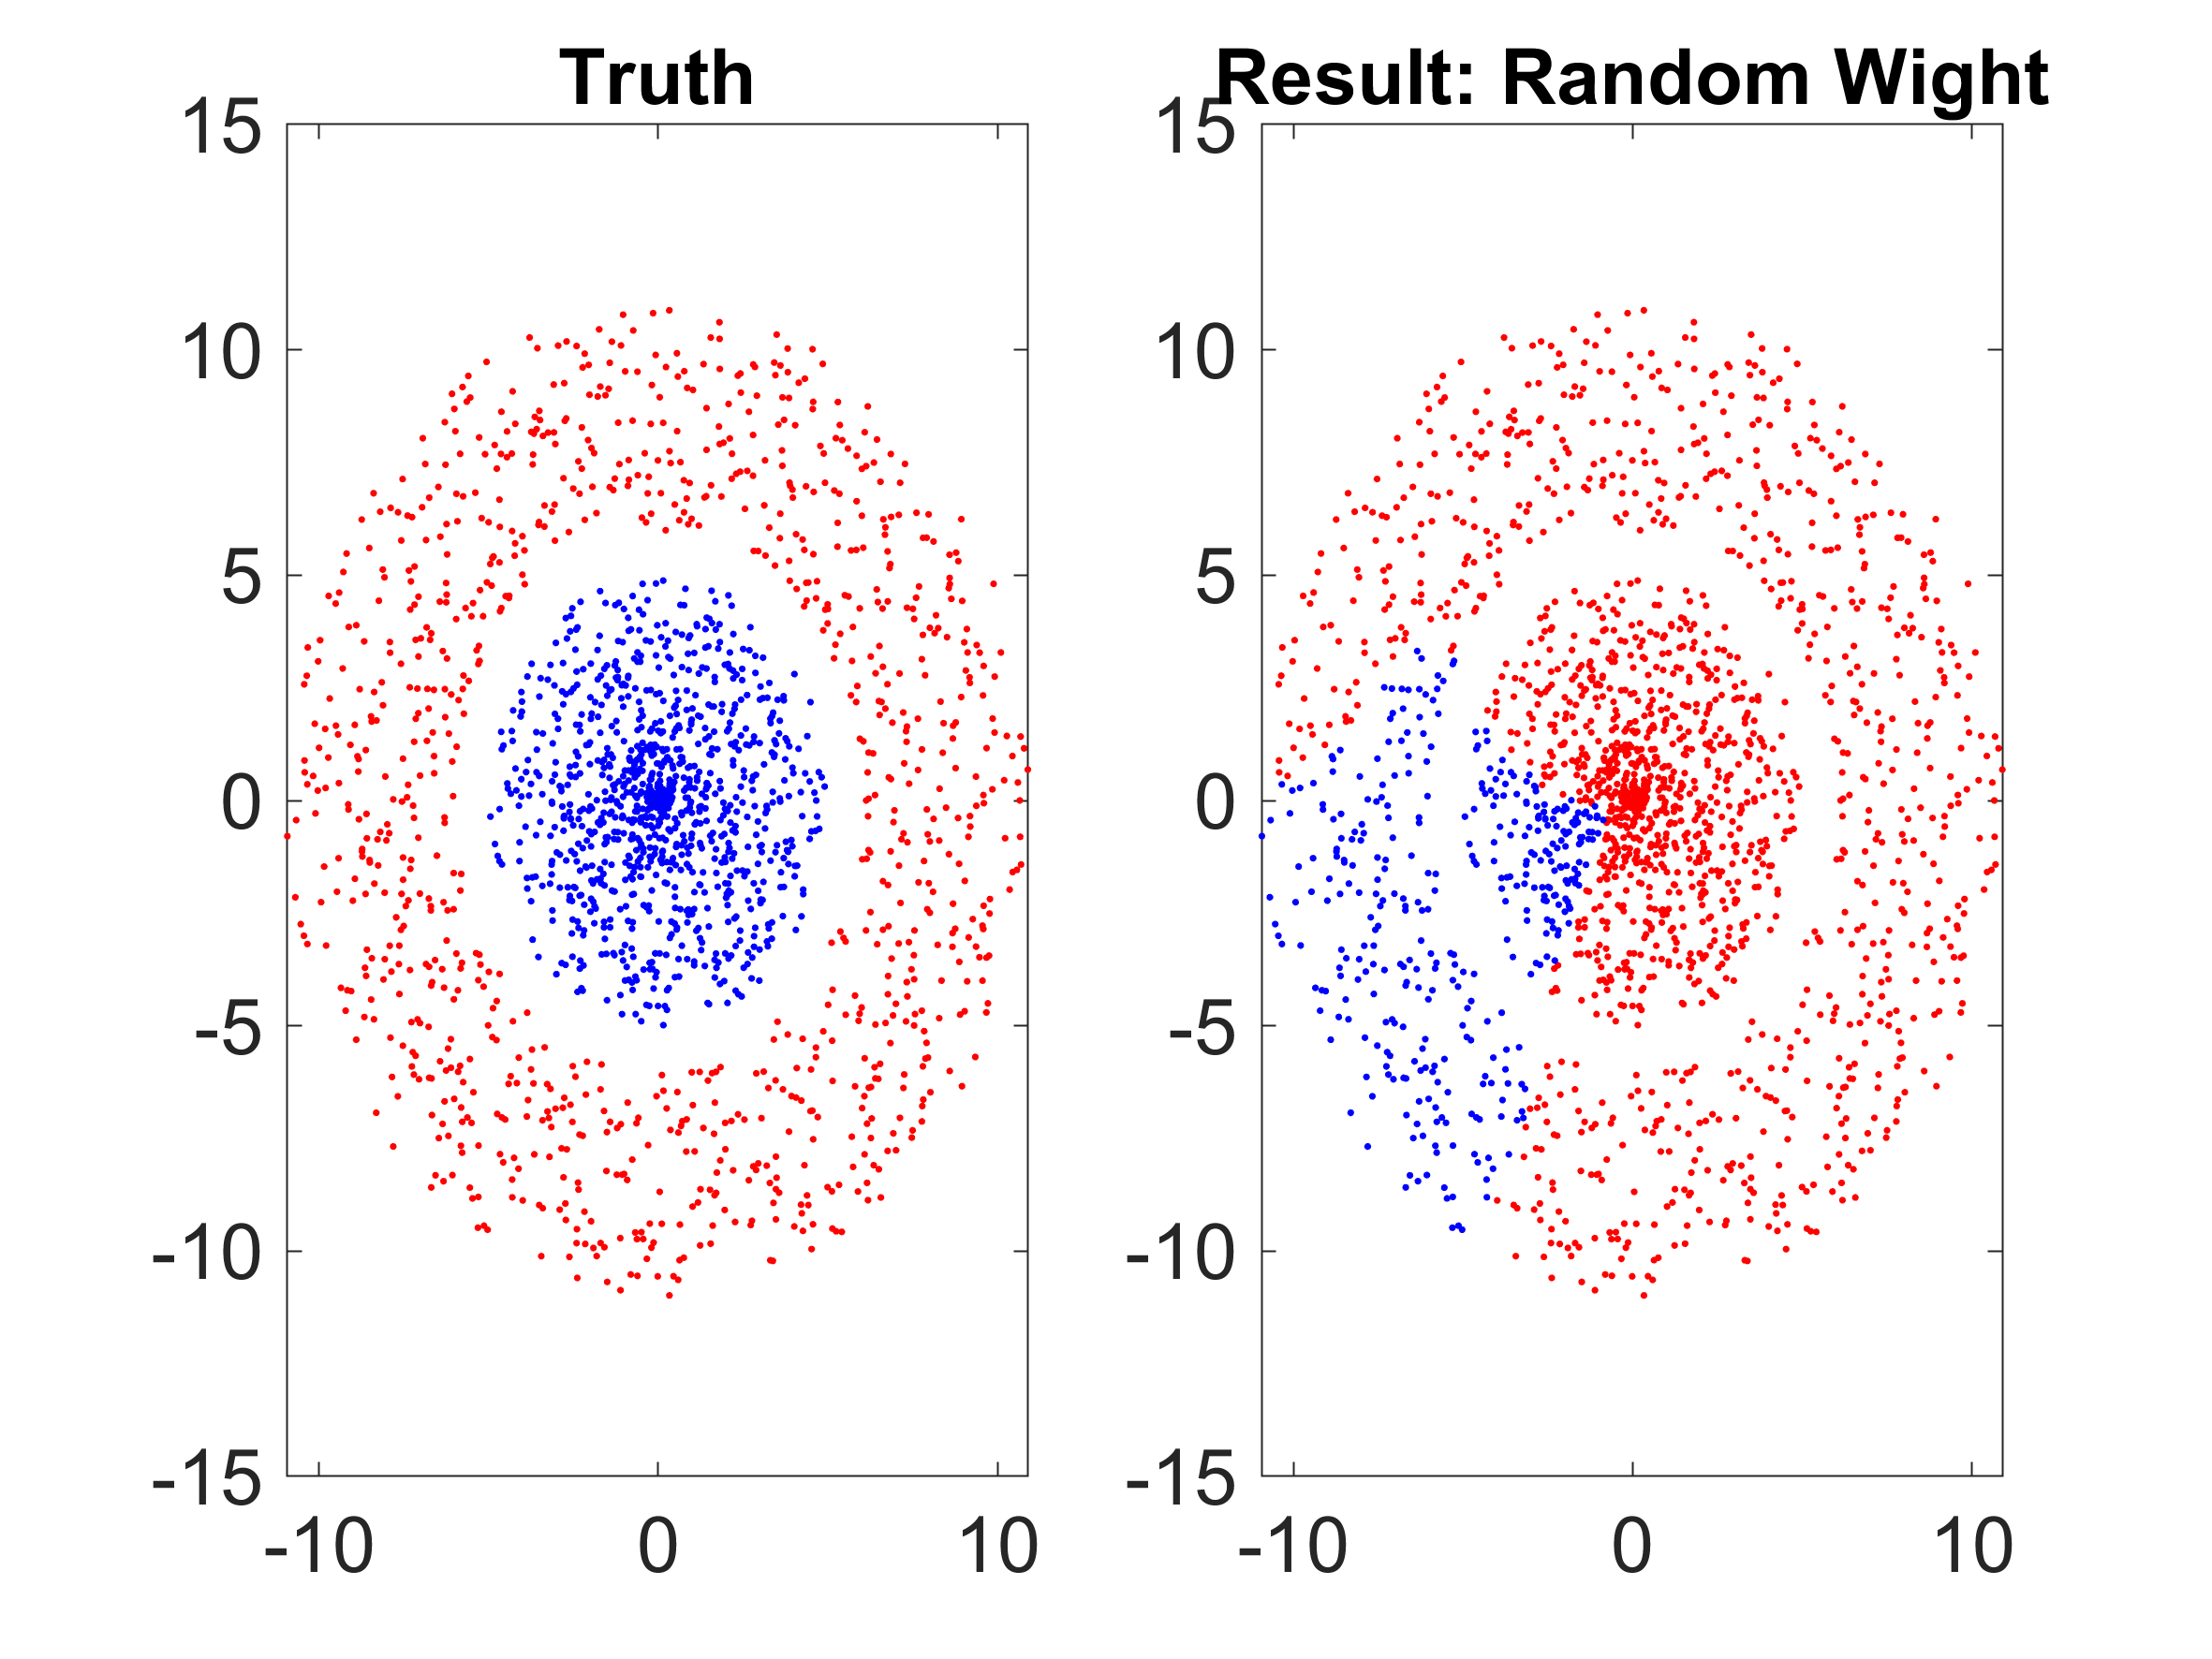
\includegraphics[scale=0.4]{figures/ex1_1.png}
			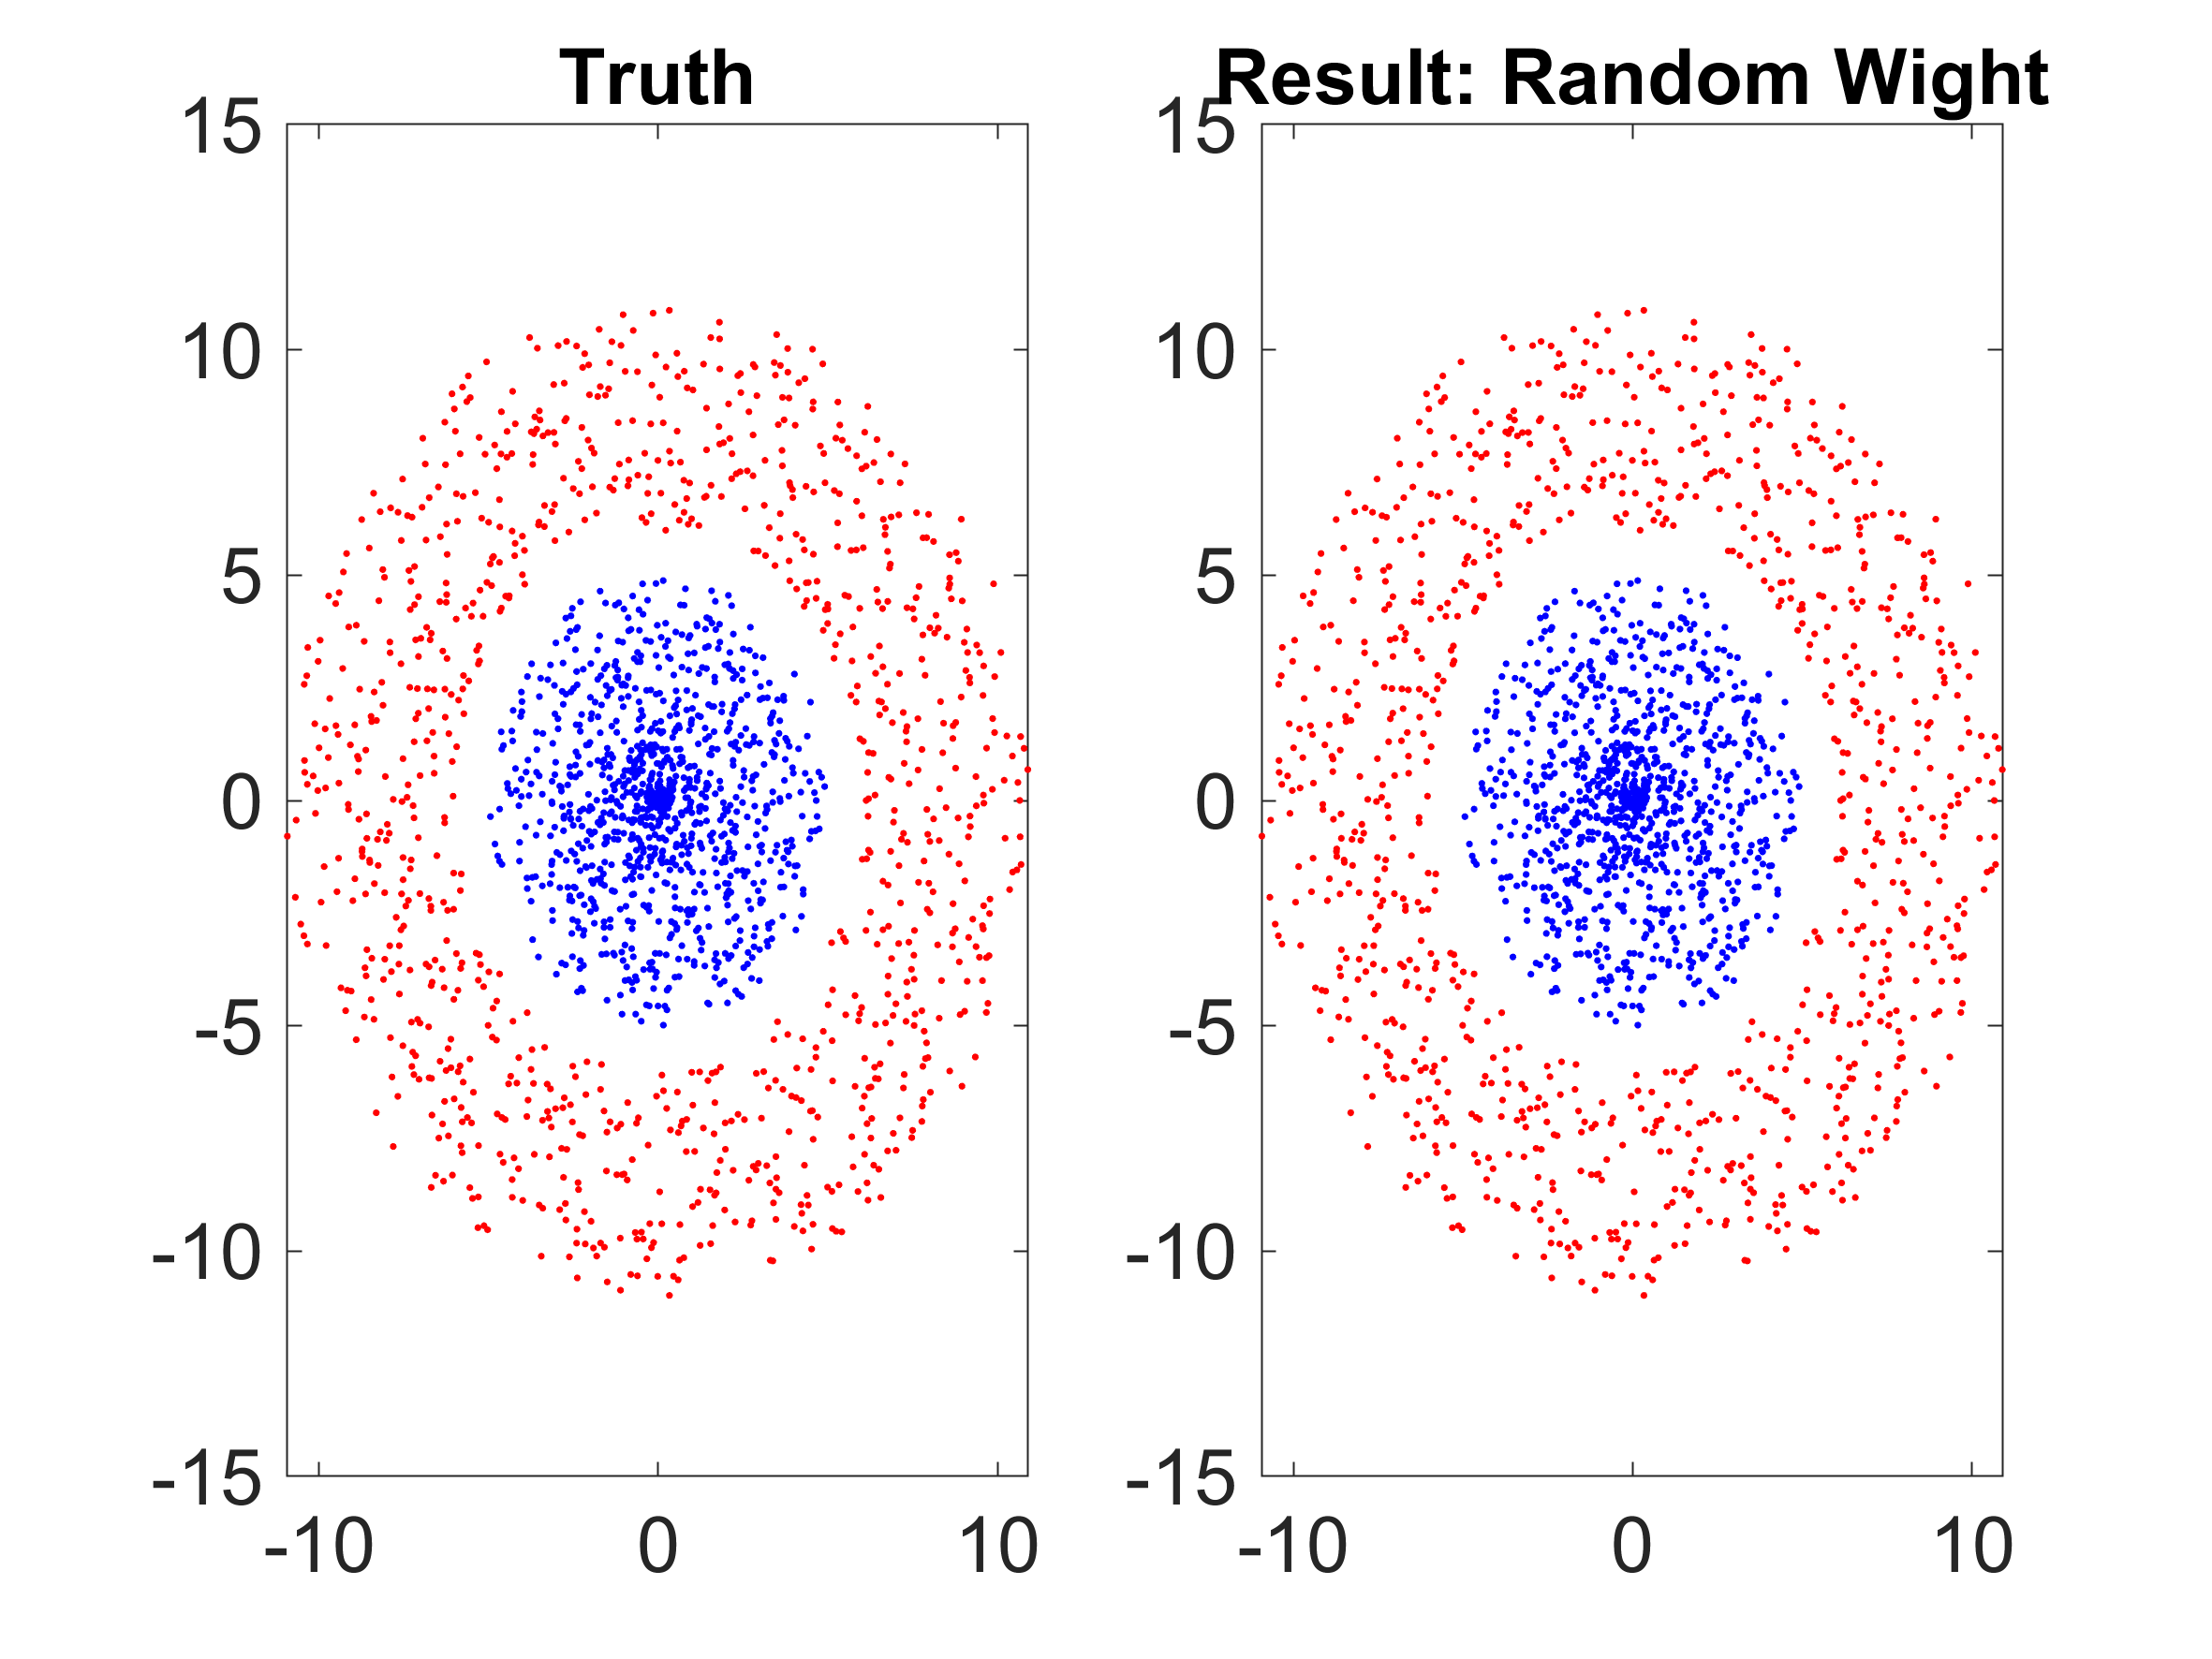
\includegraphics[scale=0.4]{figures/ex1_2.png}
	}} 
	\caption{Point cloud segmentation results: left image shows the segmentation result after initialization using random wieghts, while right image shows the final segmentation result.}
\end{figure*}
\begin{figure*}[thpb]
	\setlength{\fboxrule}{0.0pt}      
	\framebox{\parbox{6.5in}{
			\centering
			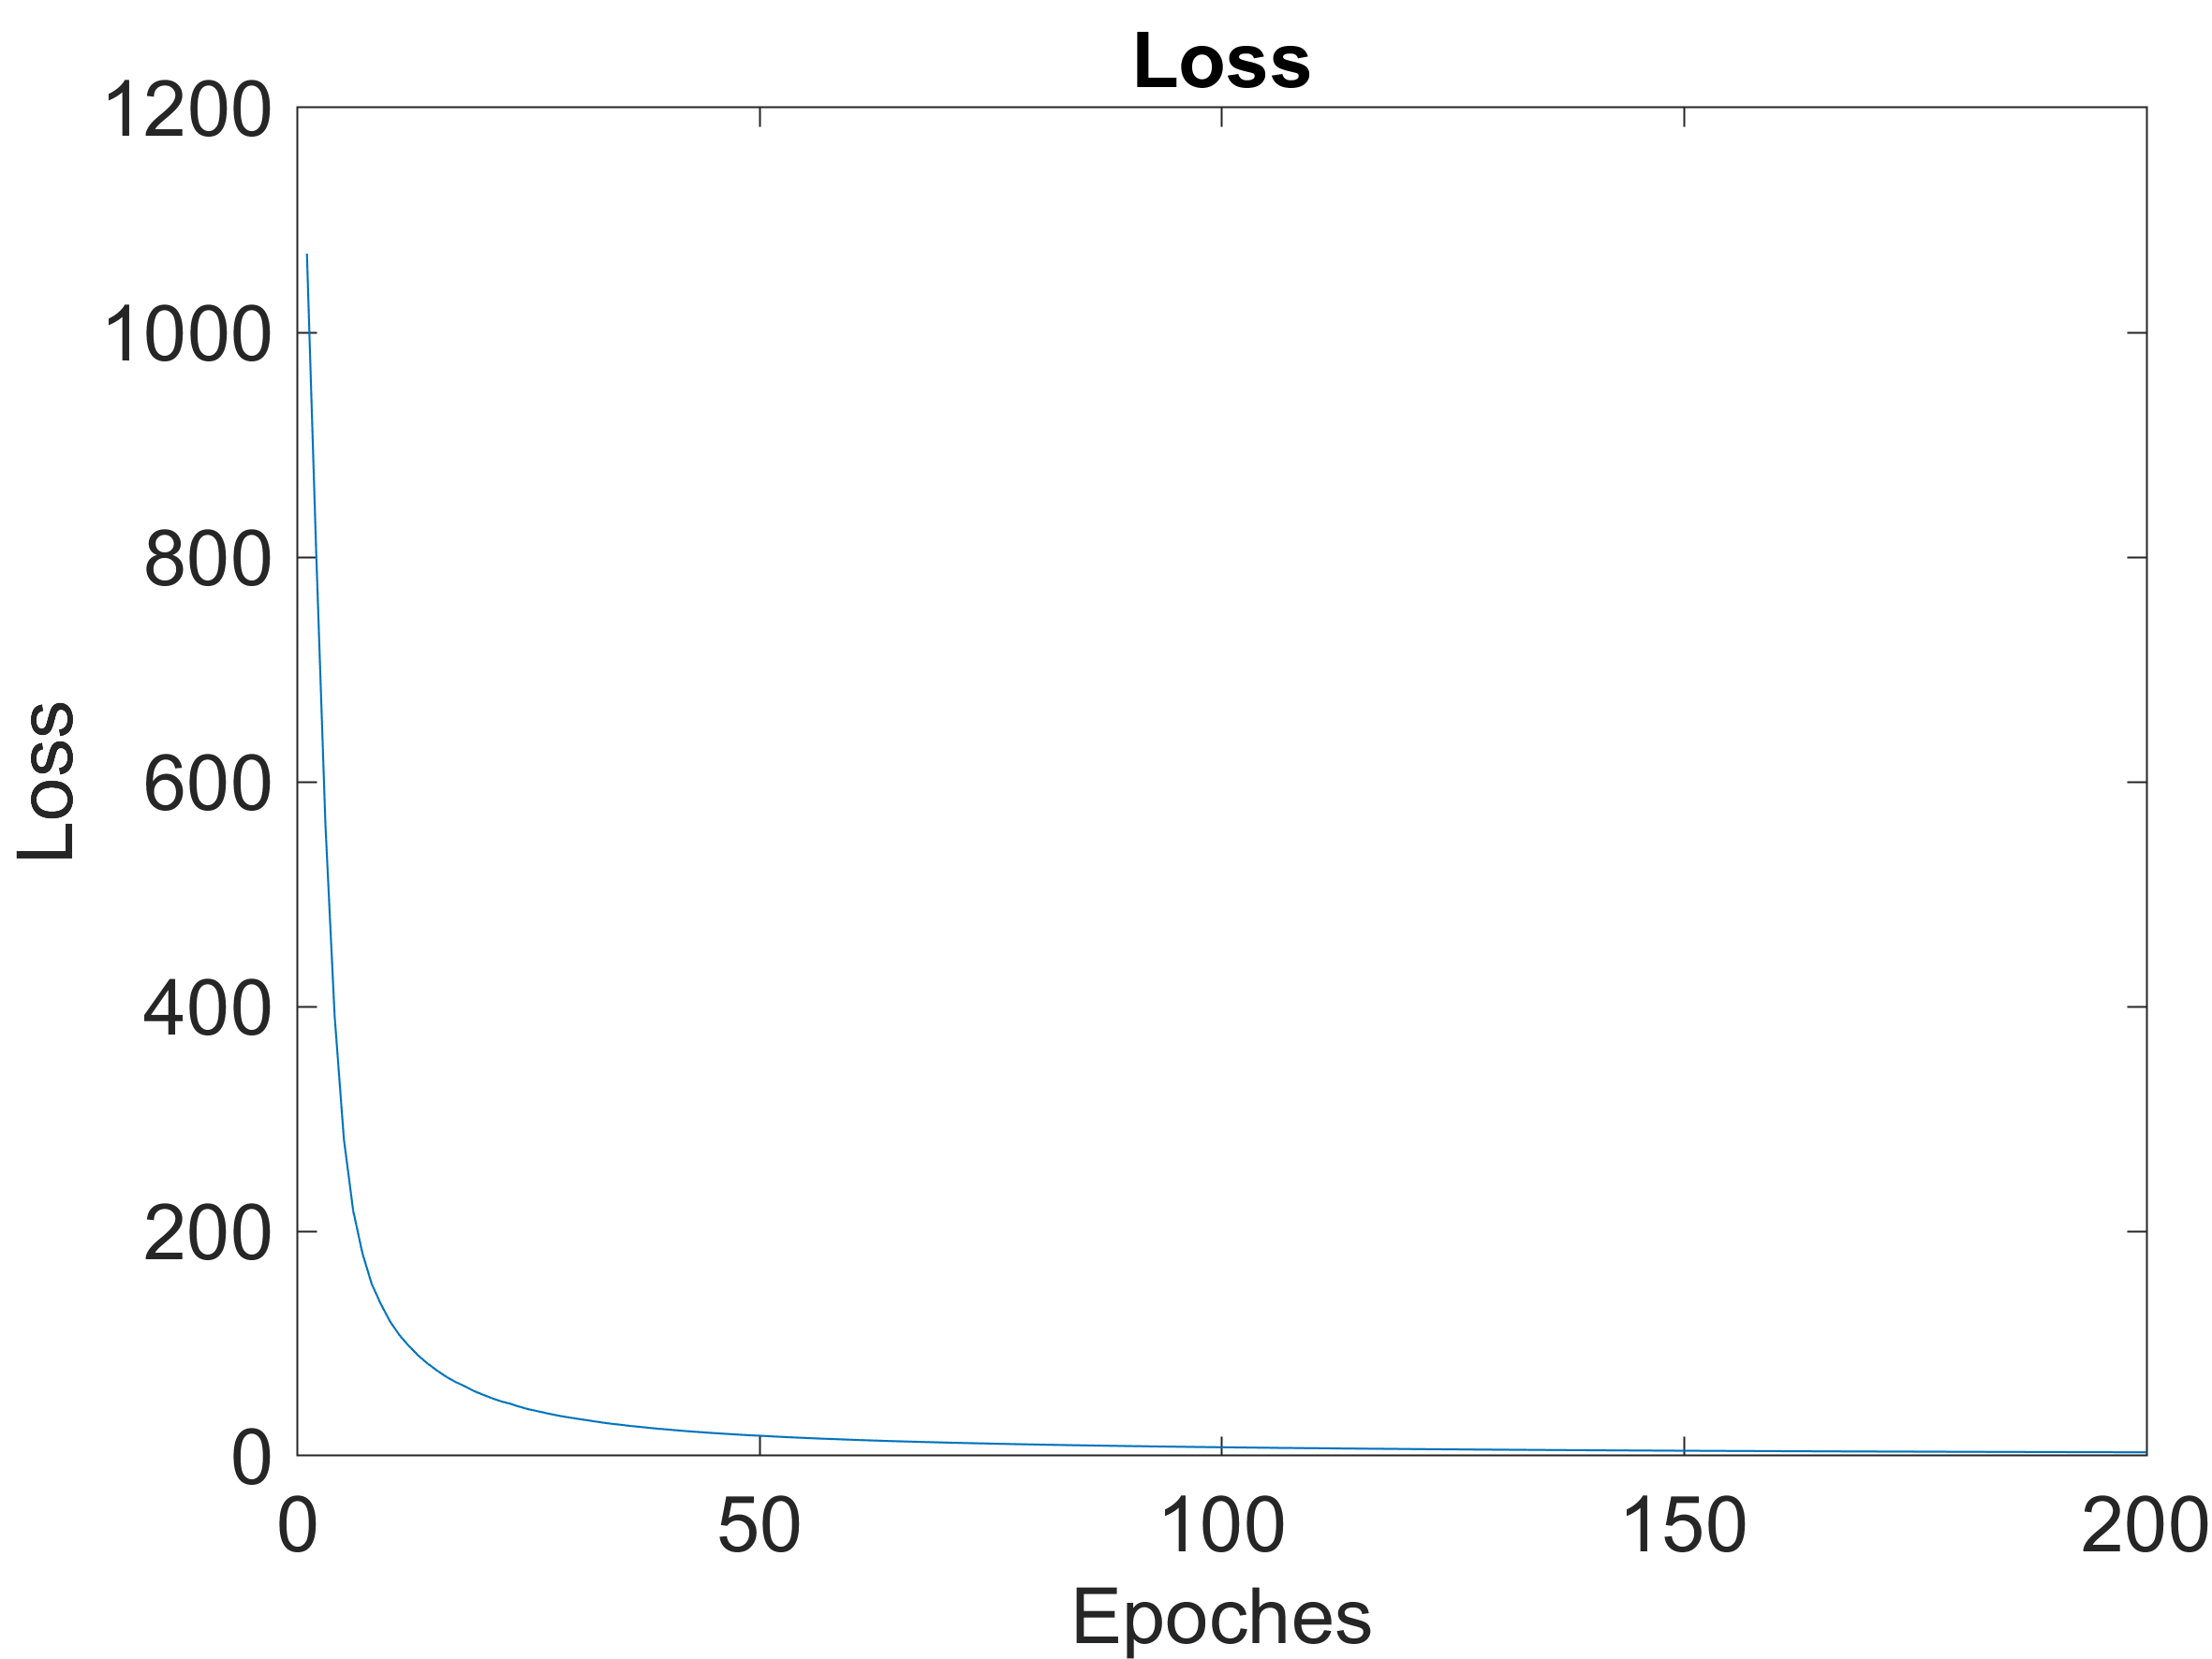
\includegraphics[scale=0.4]{figures/ex1_3.png}
			\hspace{10mm}
			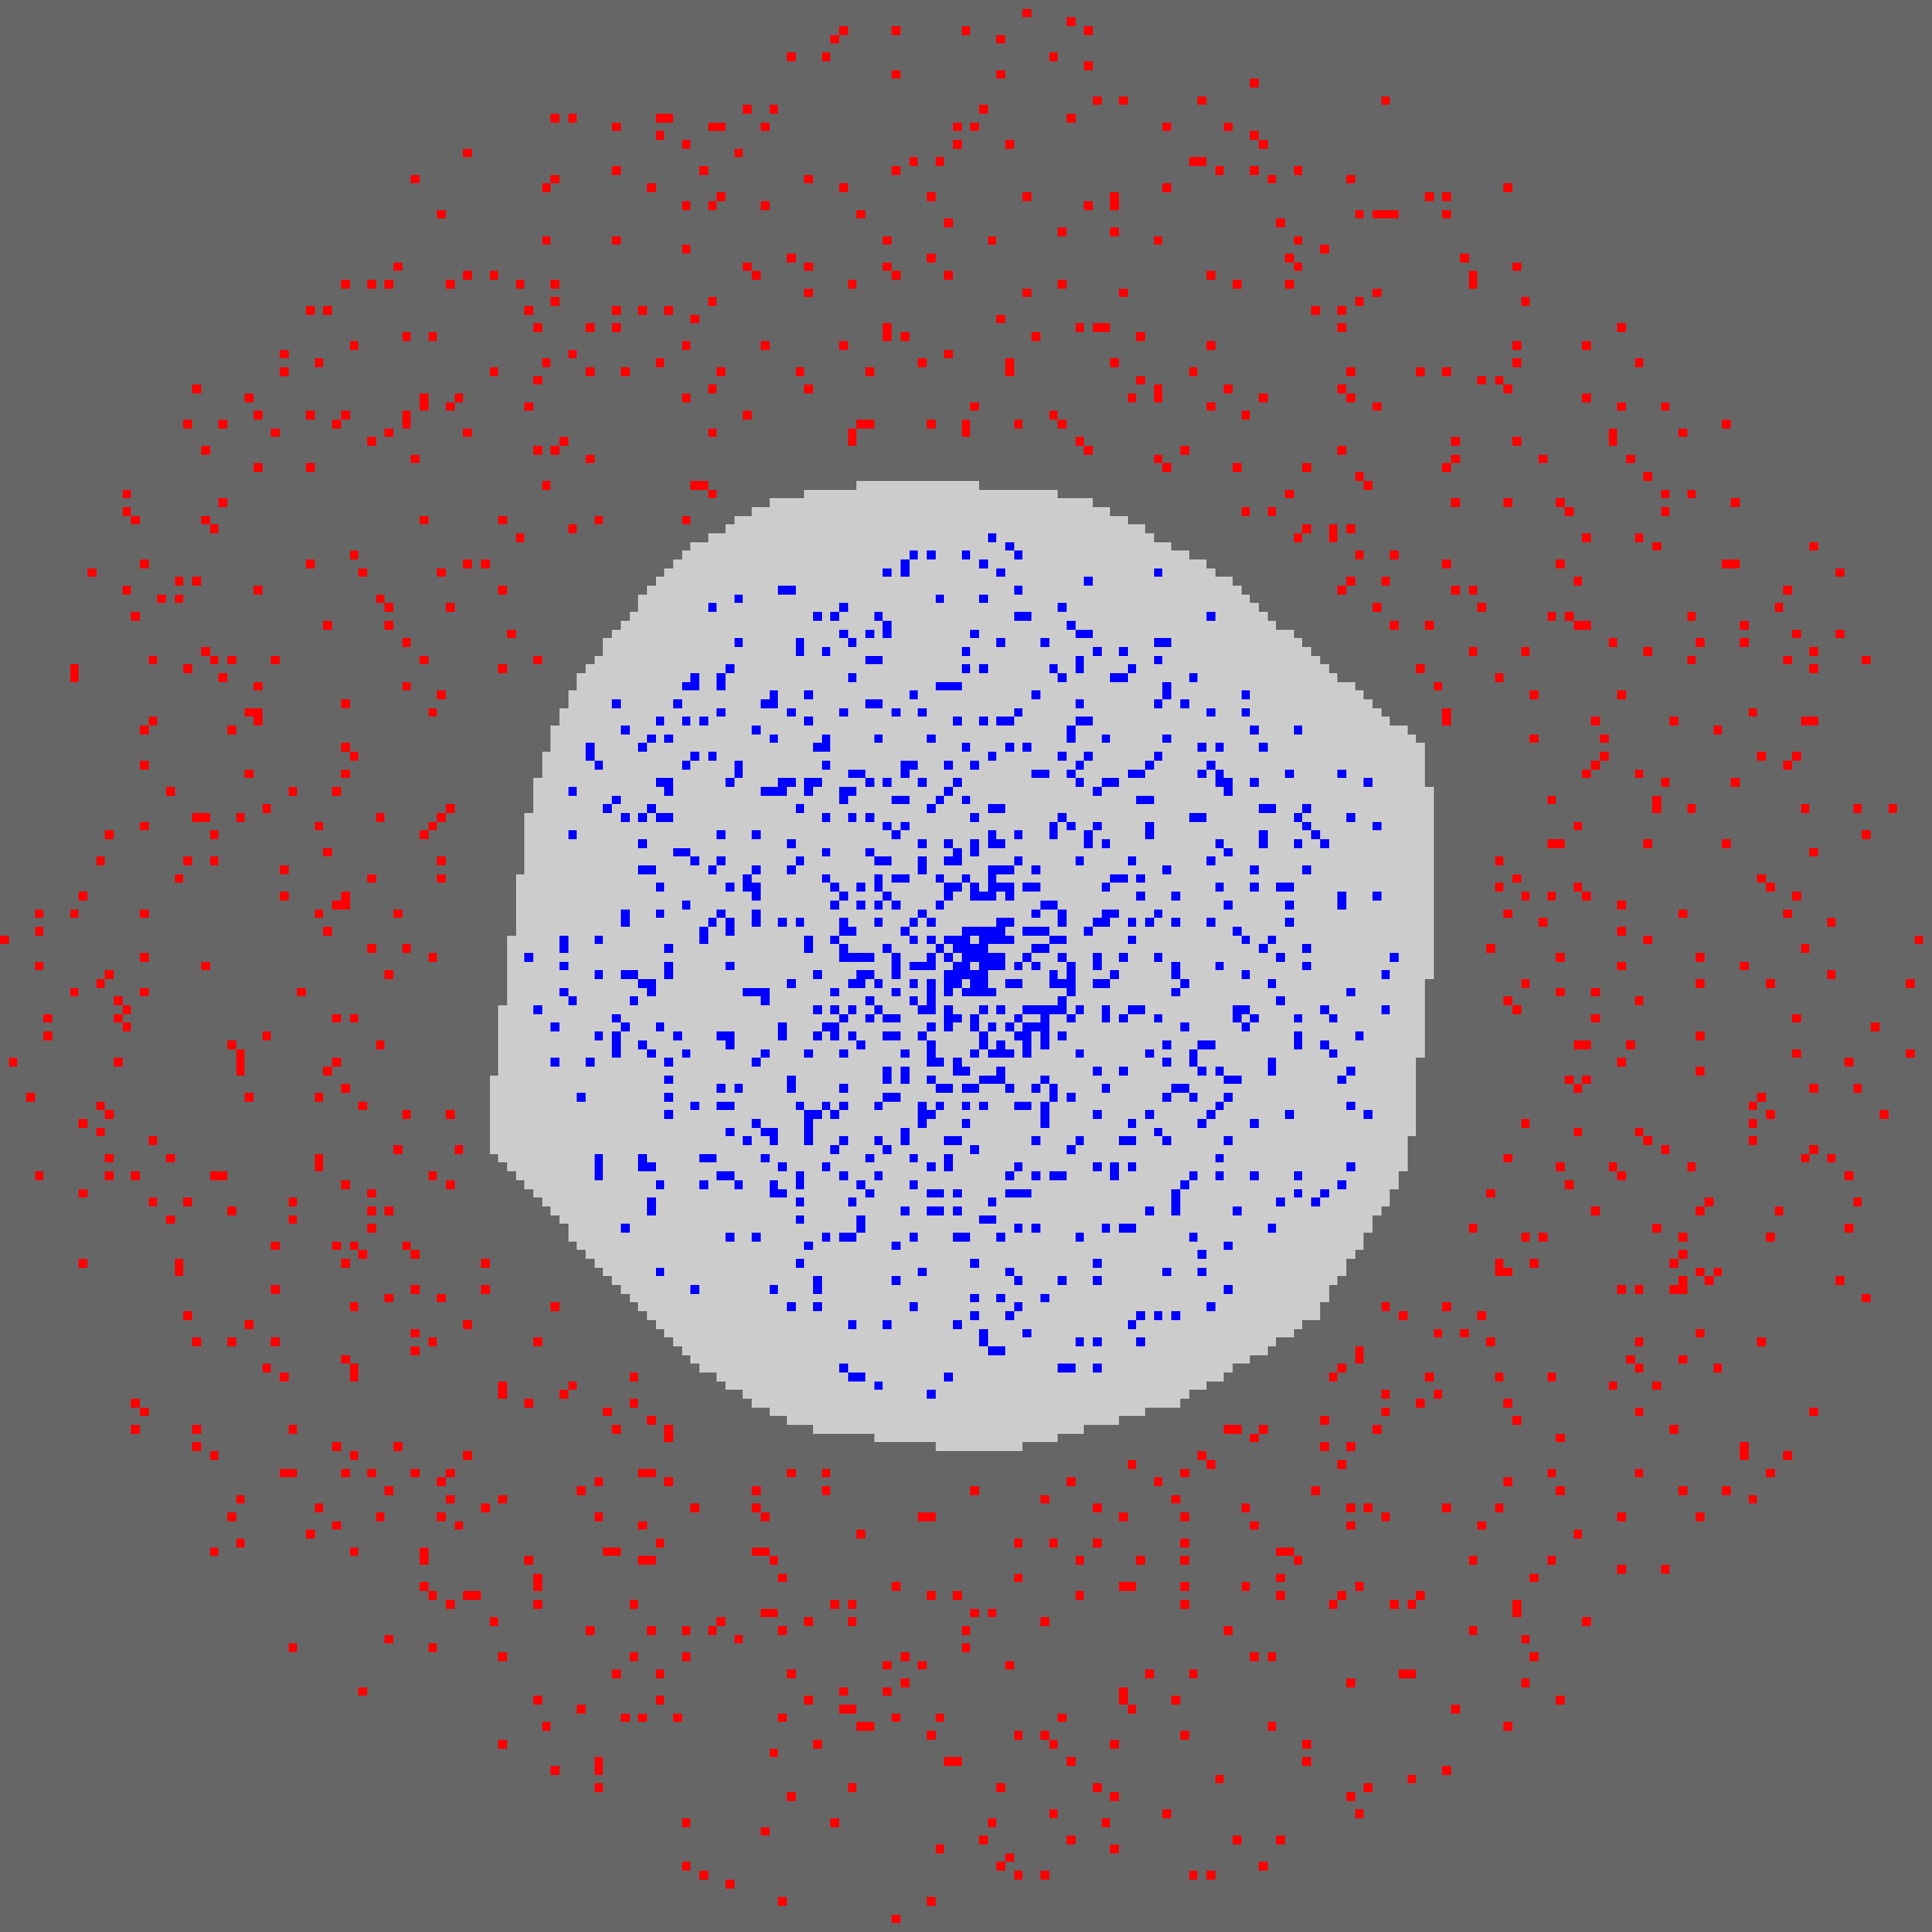
\includegraphics[scale=0.3]{figures/ex1_4.png}
	}} 
	\caption{Left image shows the training loss variations with epochs. Right image shows the segmentation boundary.}
\end{figure*}
	\begin{figure*}[thtbp]
	\setlength{\fboxrule}{0.0pt}      
	\framebox{\parbox{6.5in}{
			\centering
			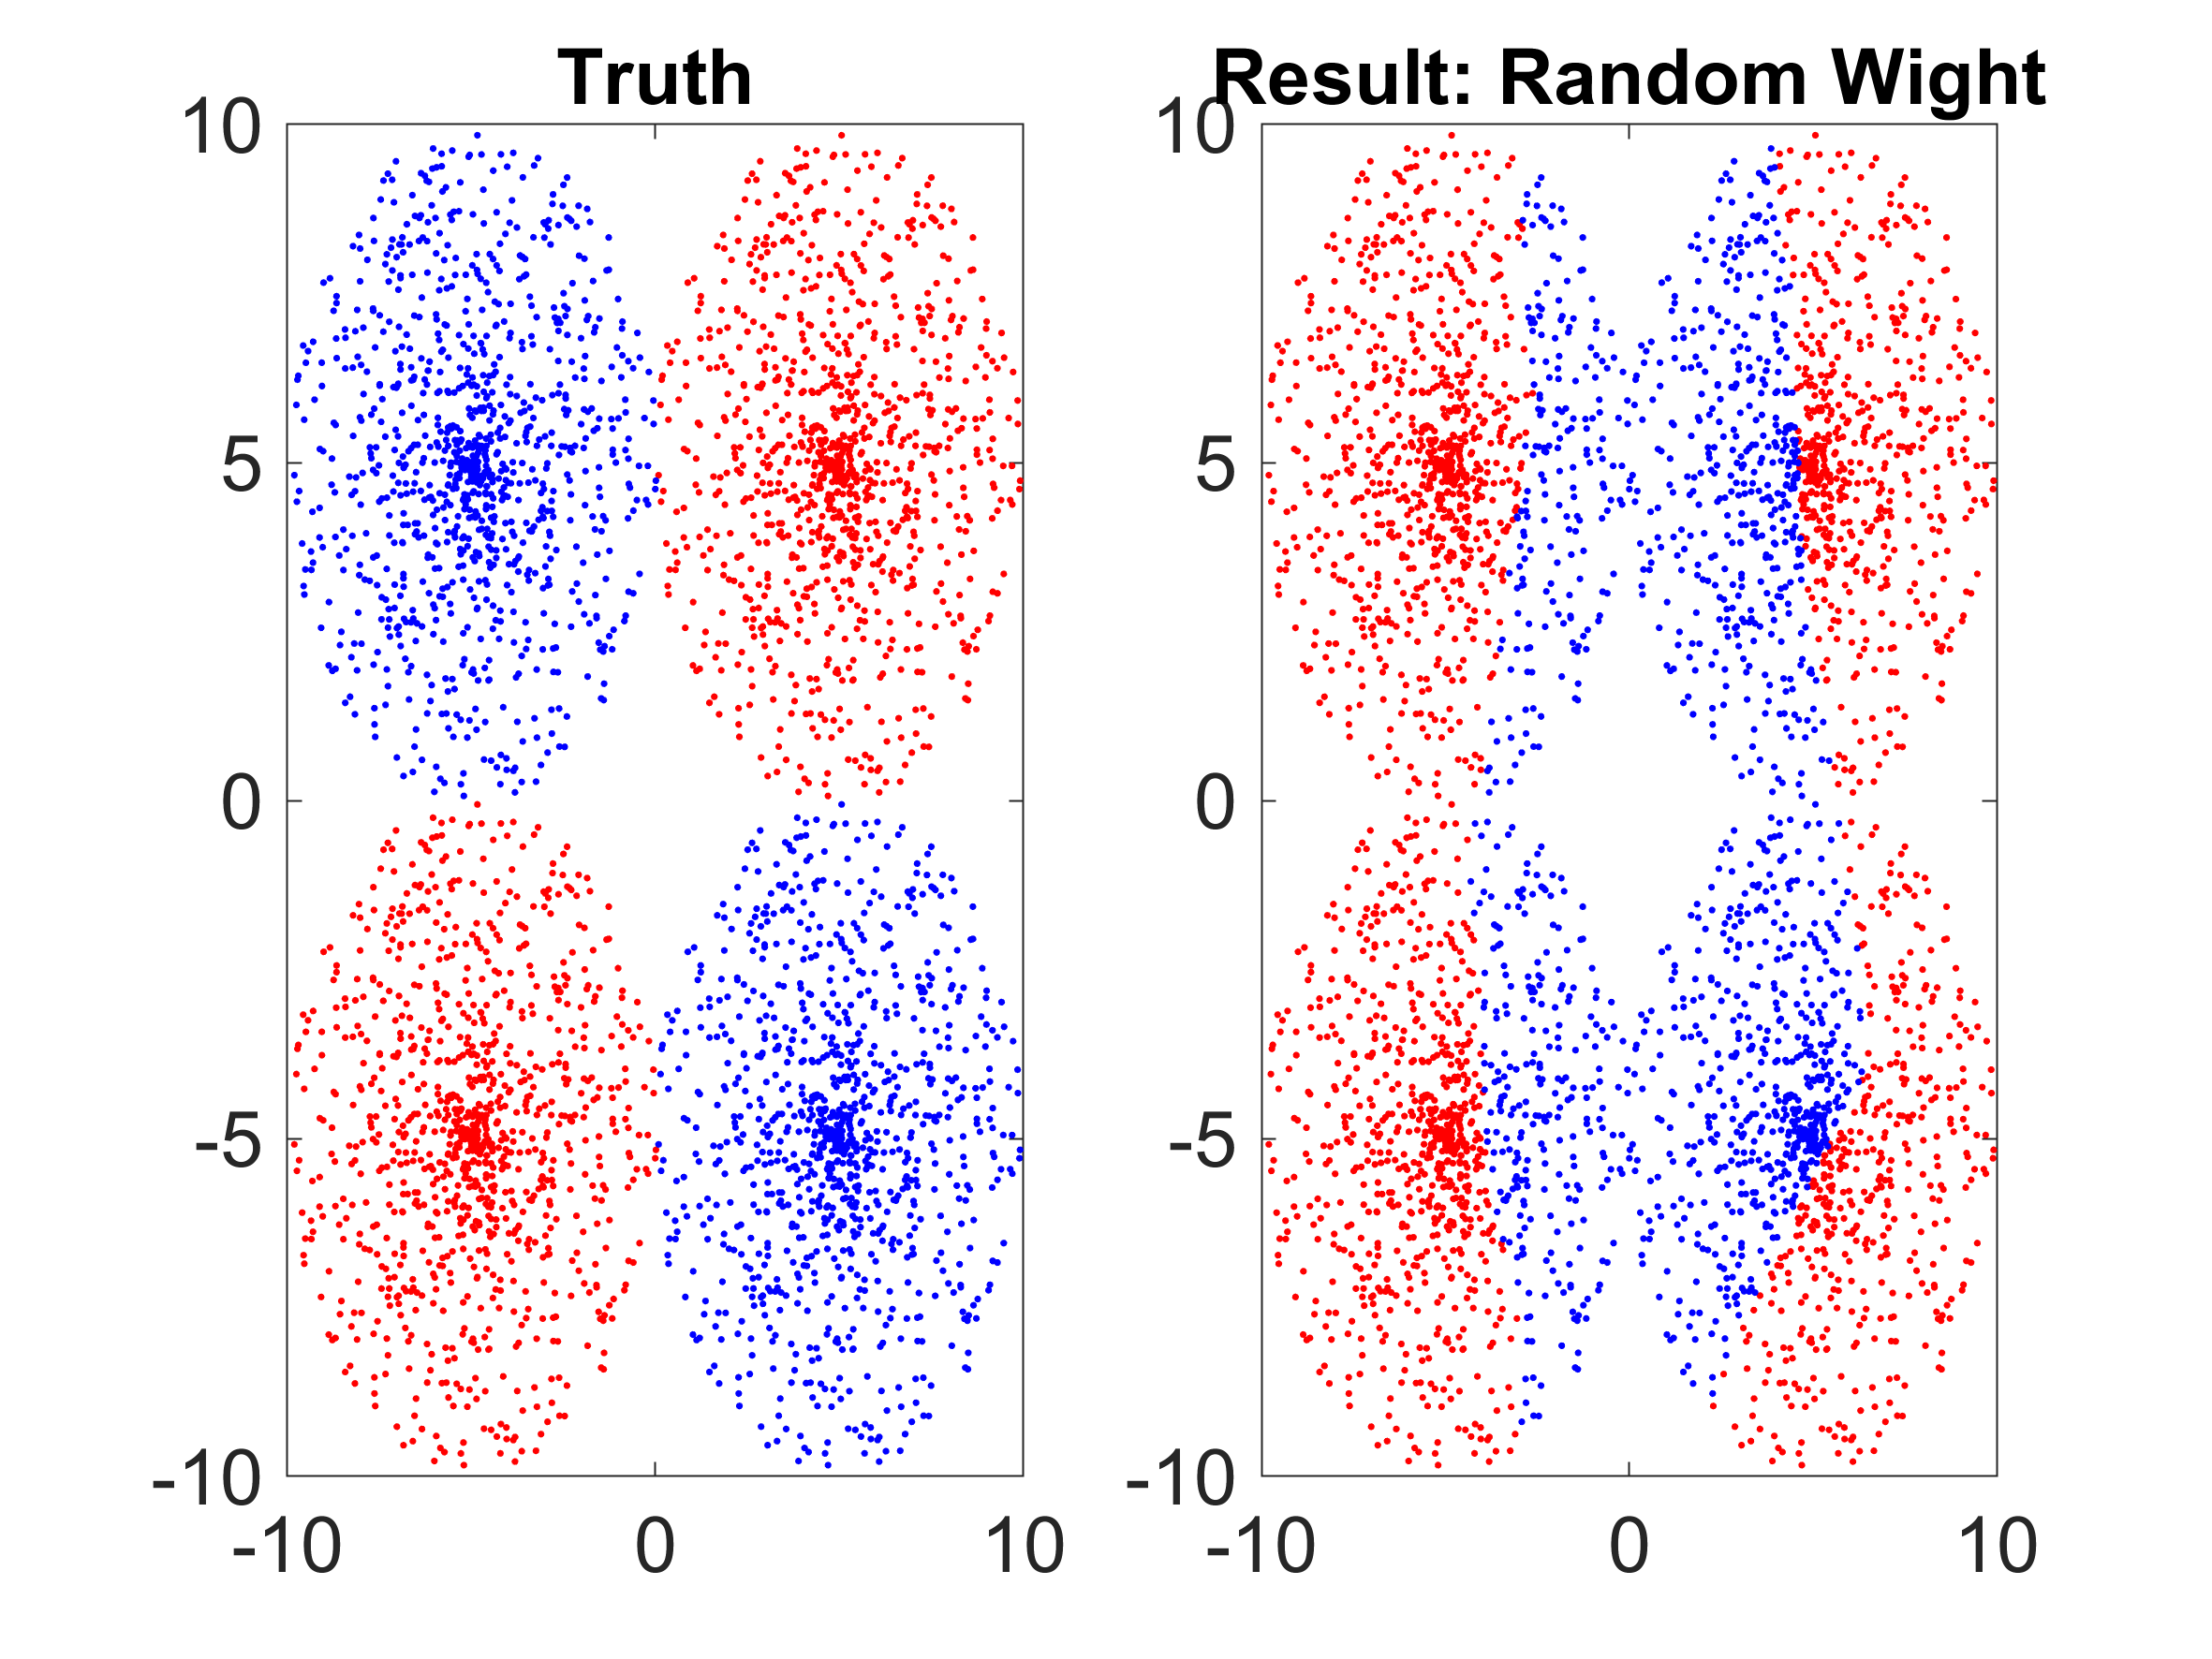
\includegraphics[scale=0.4]{figures/ex3_1.png}
			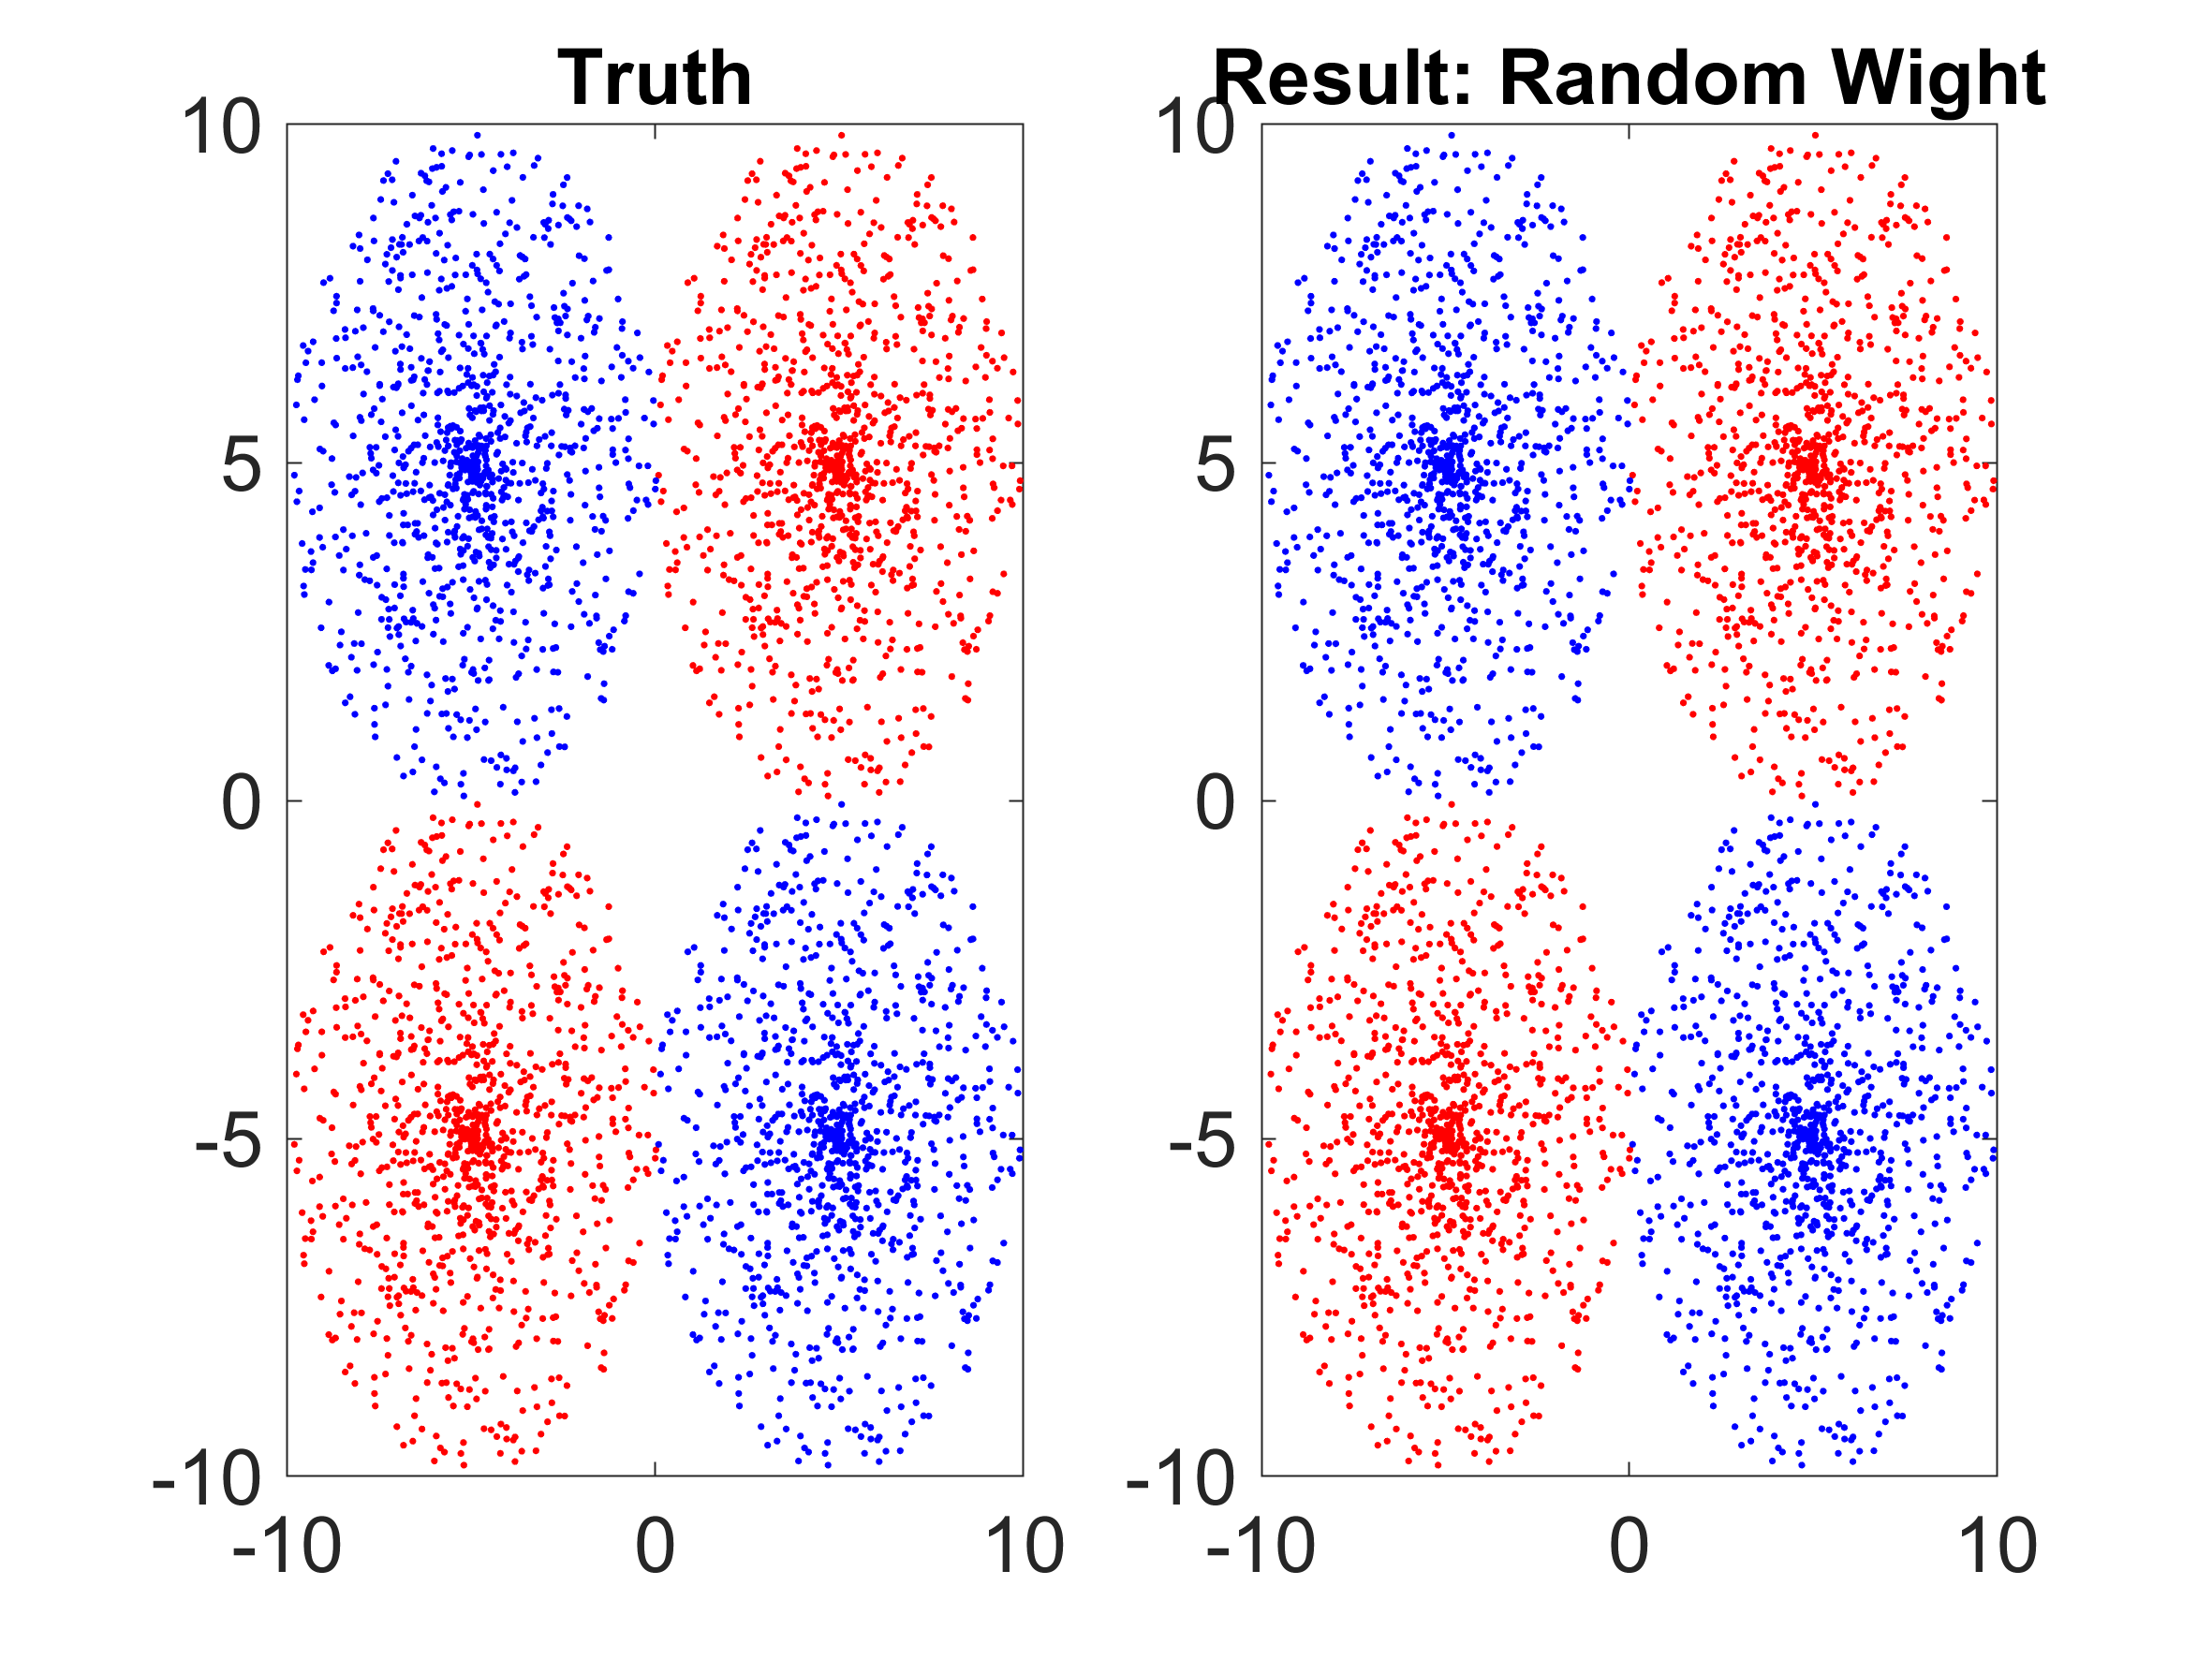
\includegraphics[scale=0.4]{figures/ex3_2.png}
	}} 
	\caption{Point cloud segmentation results: left image shows the segmentation result after initialization using random wieghts, while right image shows the final segmentation result.}
\end{figure*}
\begin{figure*}[thpb]
	\setlength{\fboxrule}{0.0pt}      
	\framebox{\parbox{6.5in}{
			\centering
			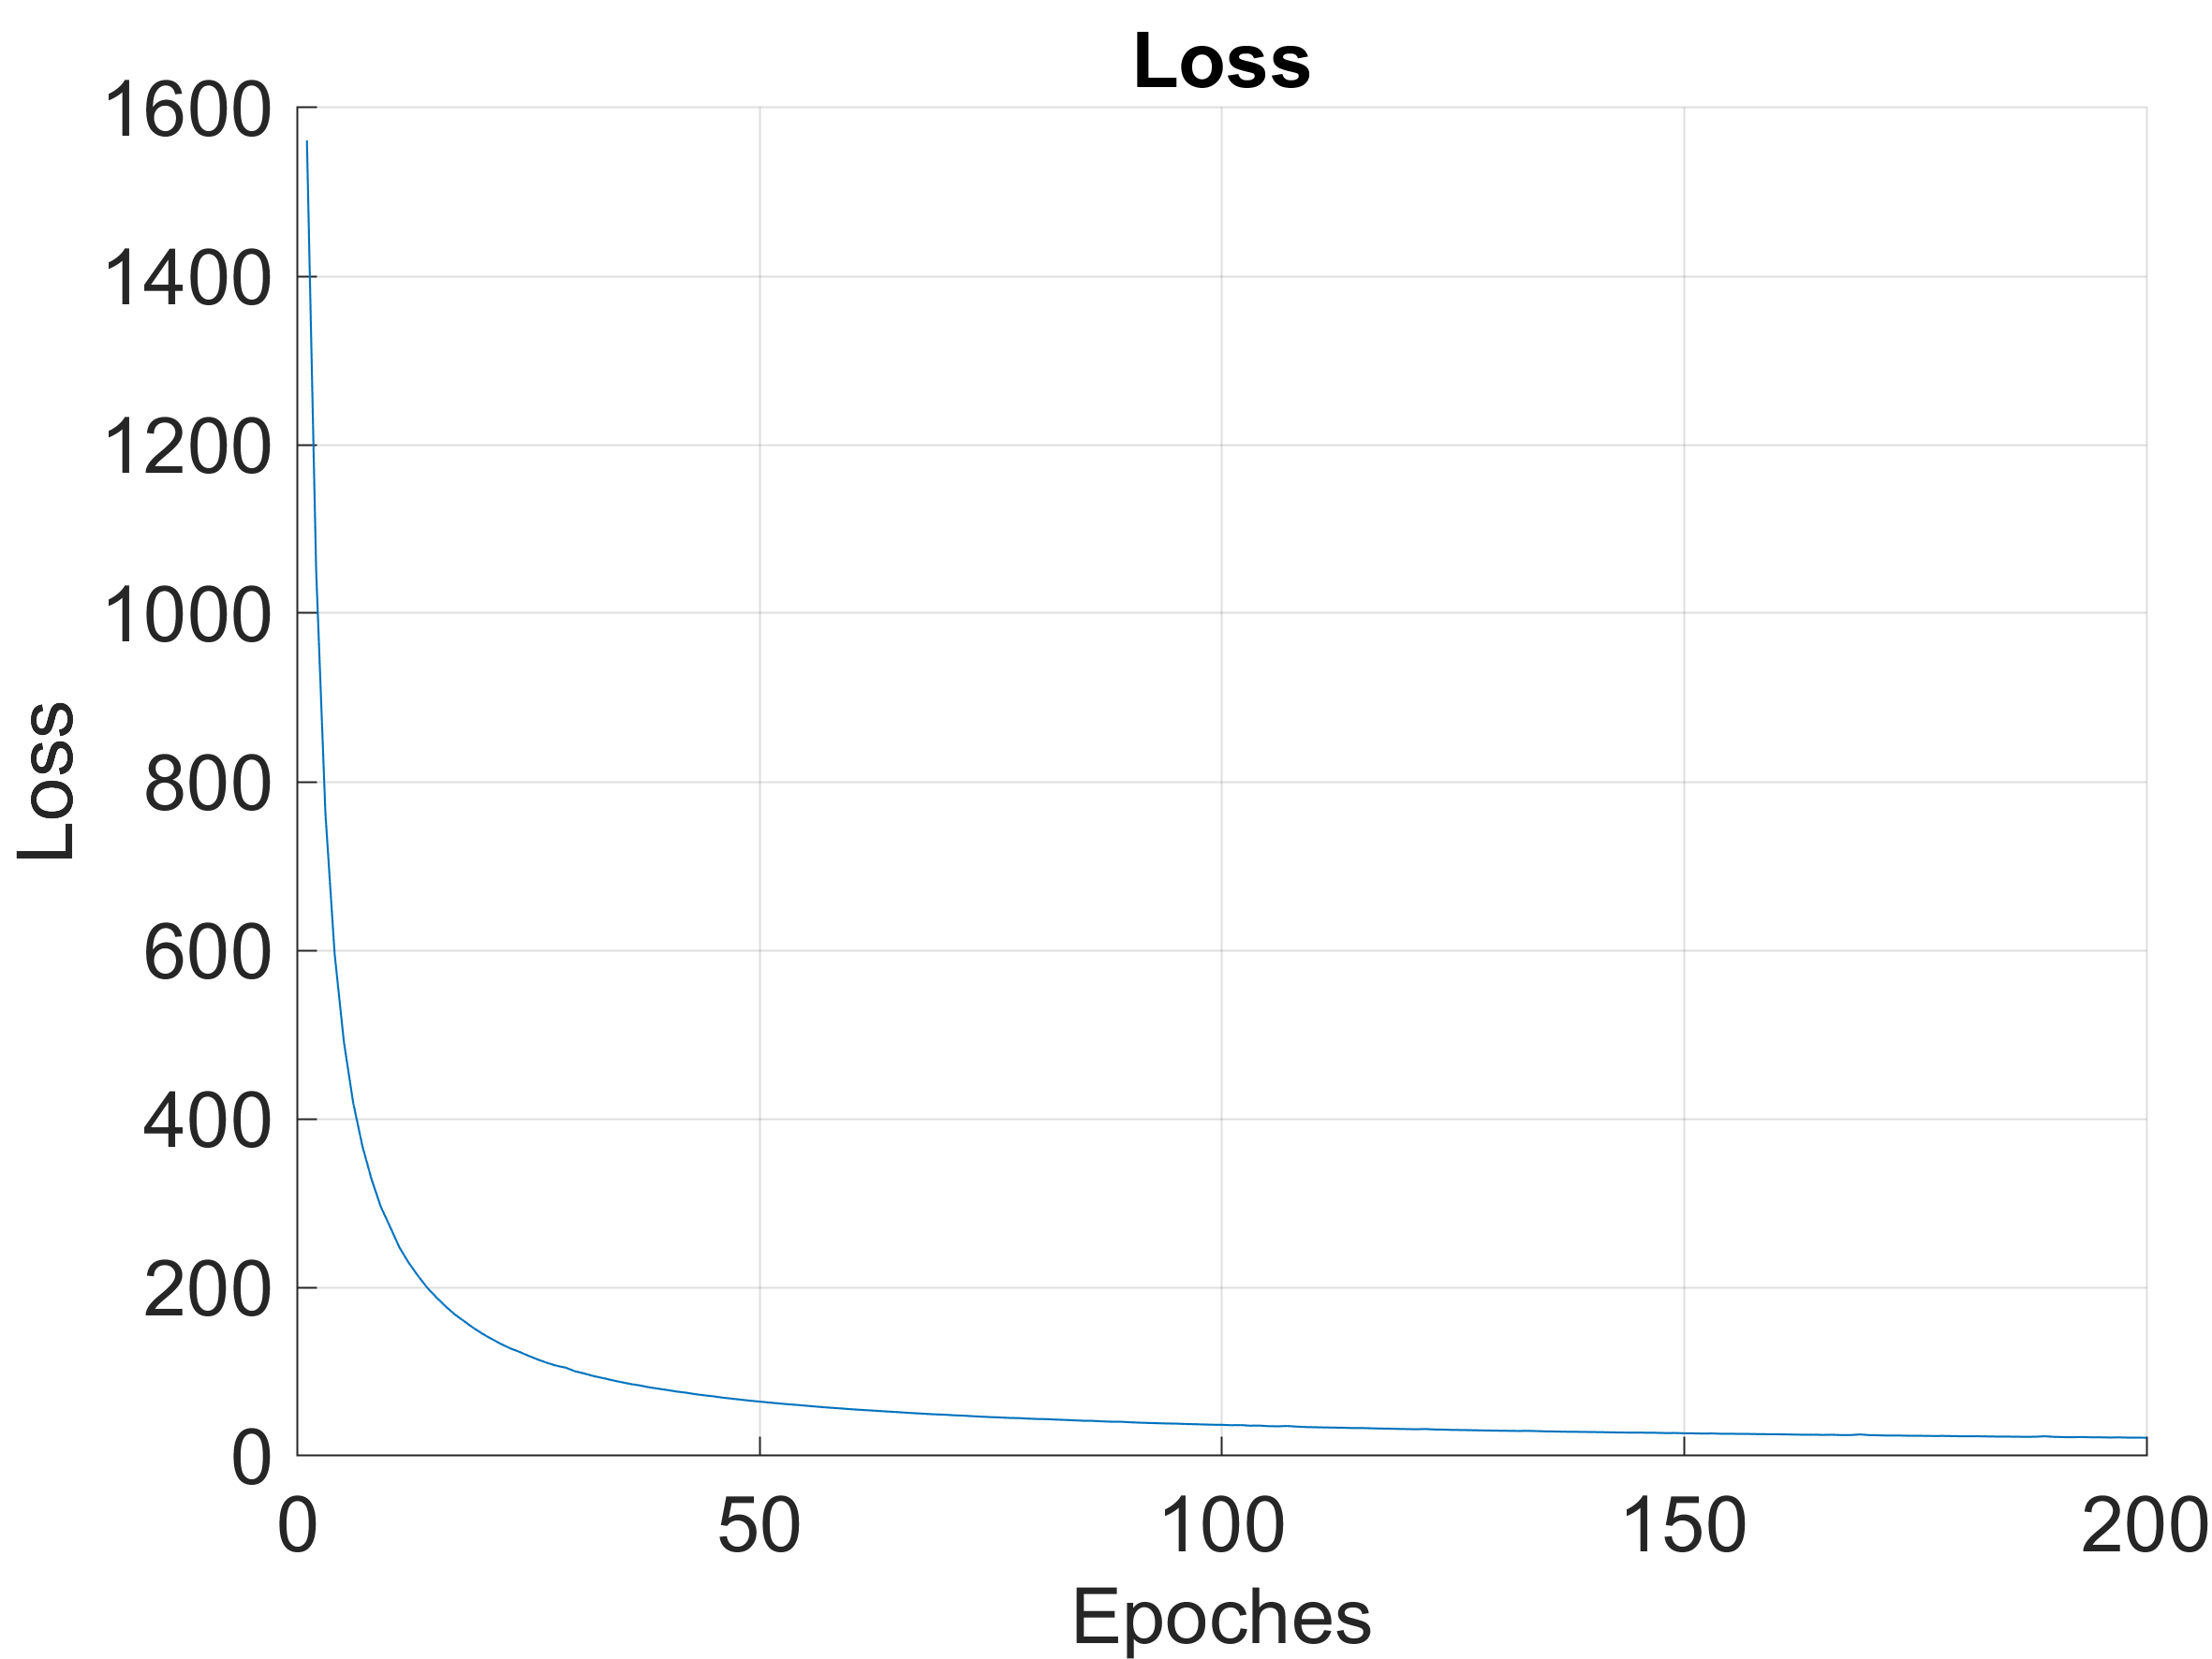
\includegraphics[scale=0.4]{figures/ex3_3.png}
			\hspace{10mm}
			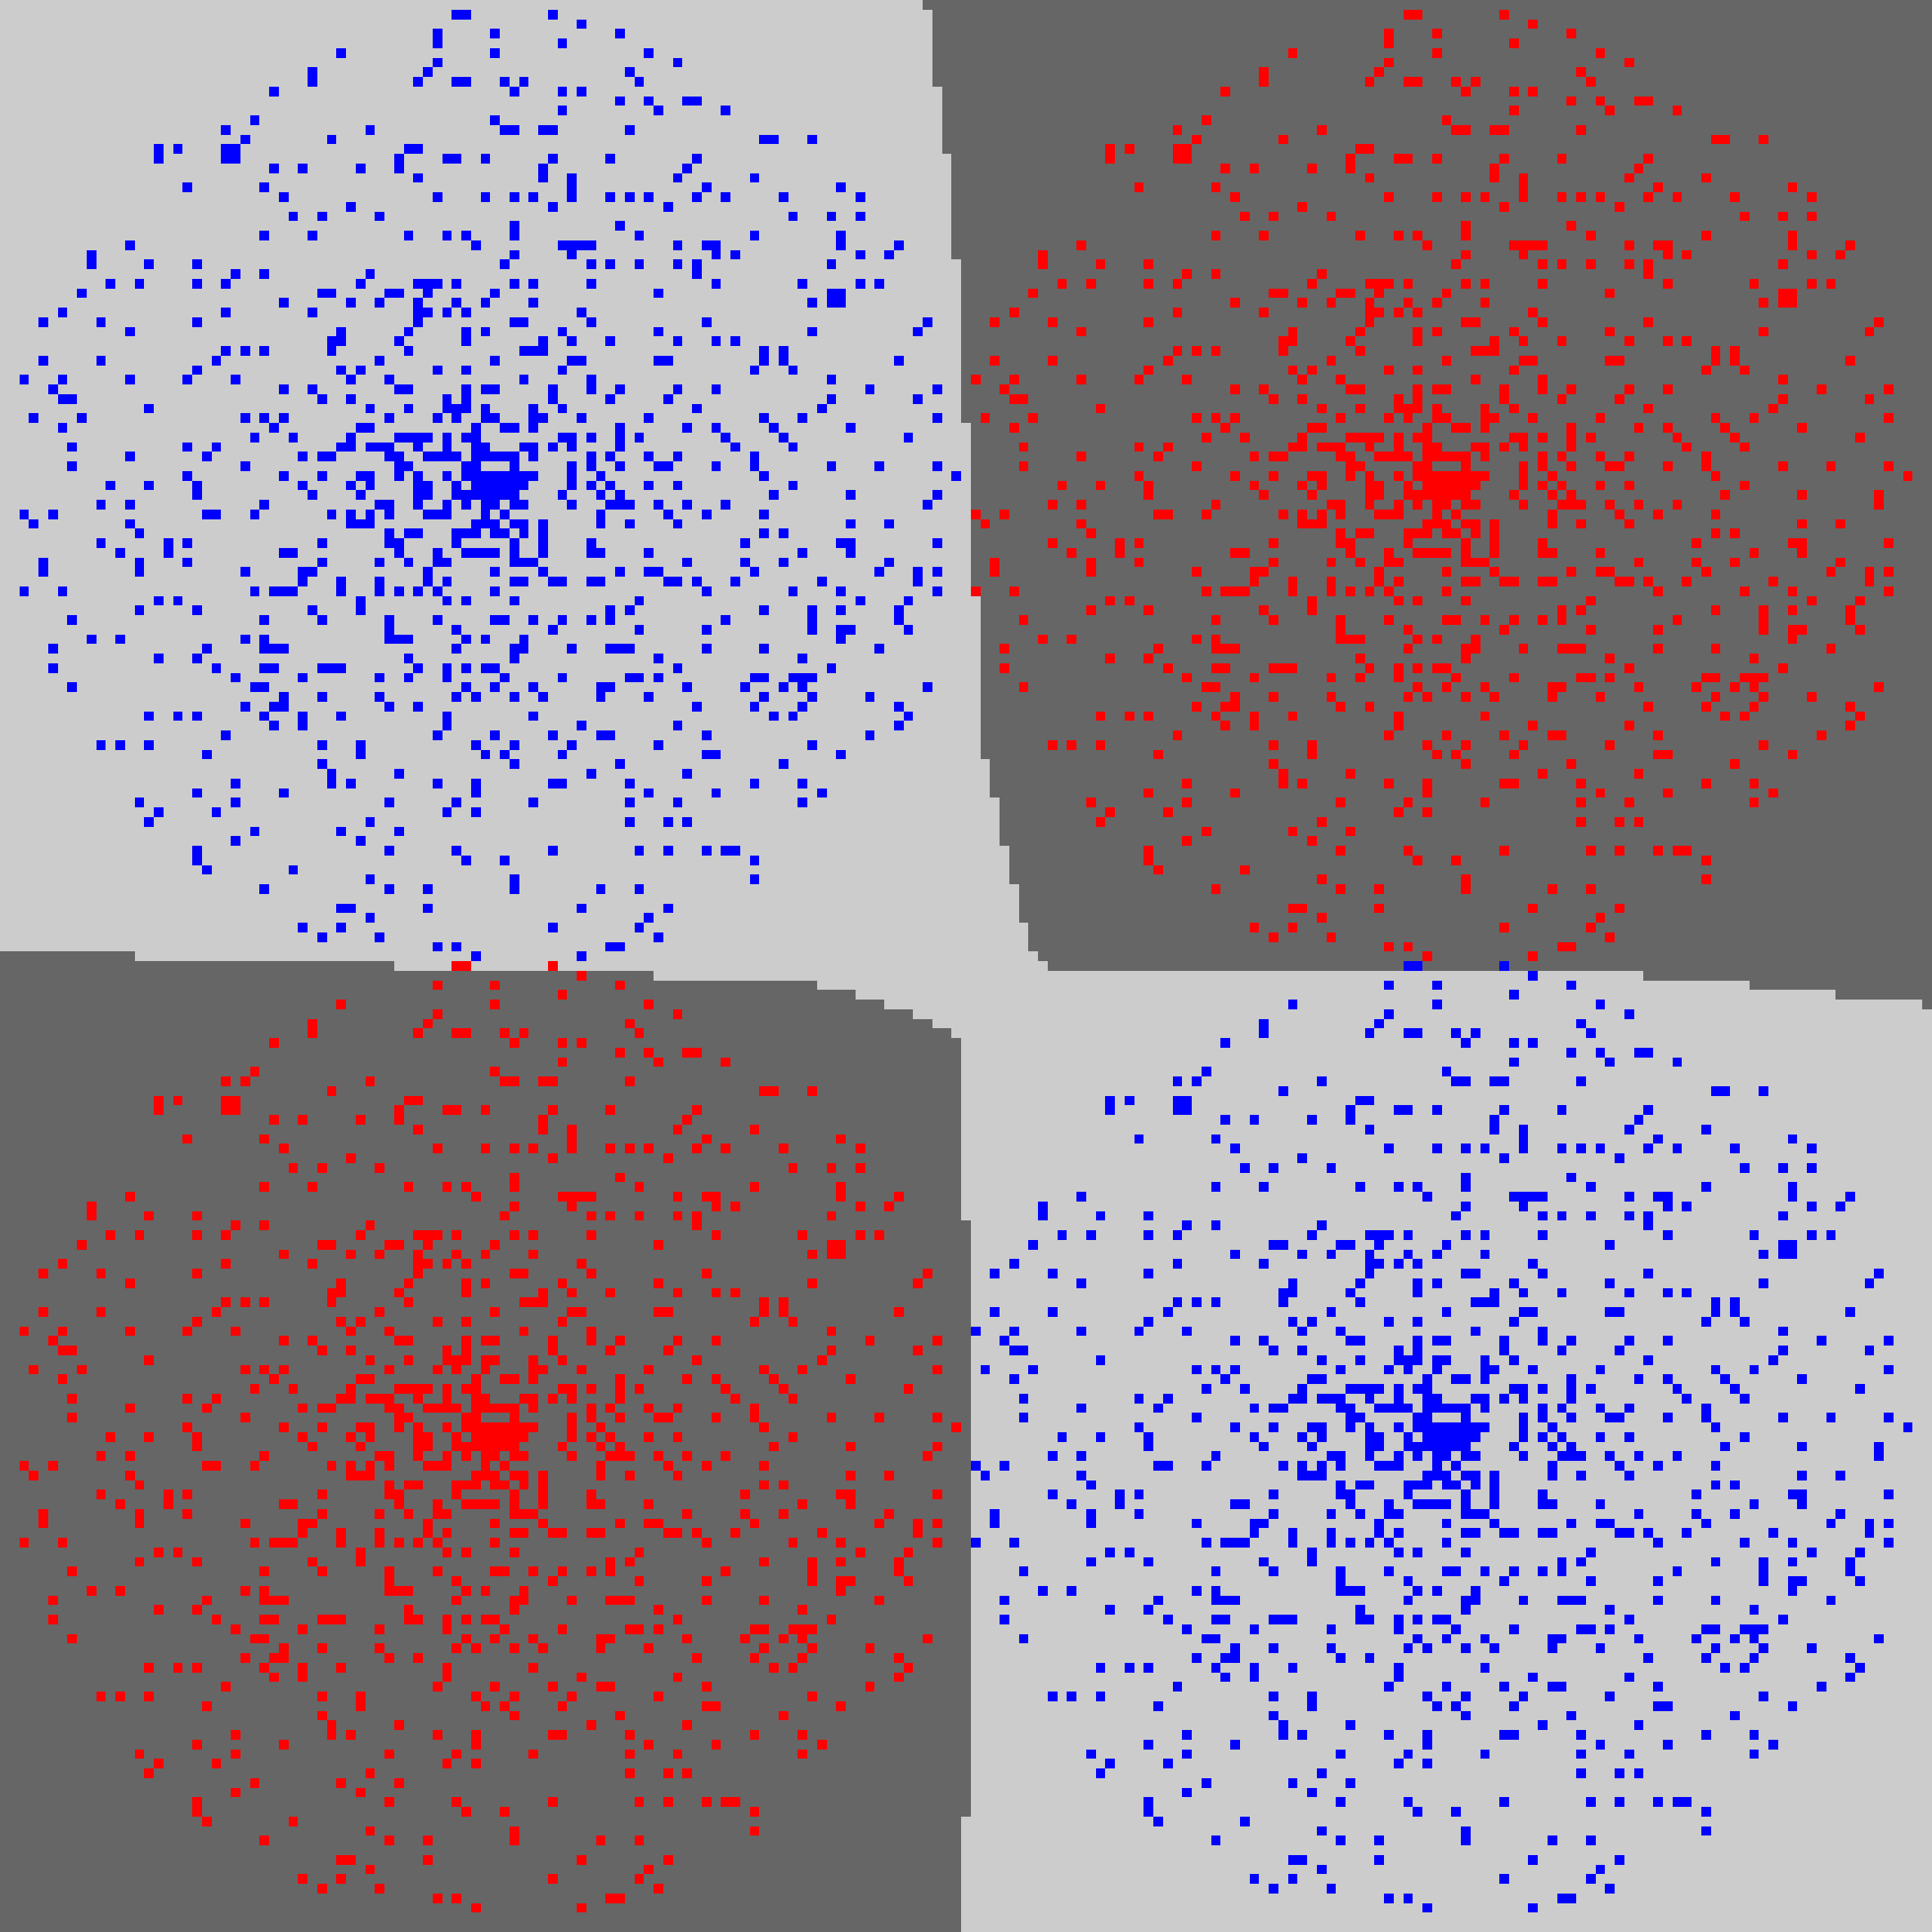
\includegraphics[scale=0.3]{figures/ex3_4.png}
	}} 
	\caption{Left image shows the training loss variations with epochs. Right image shows the segmentation boundary.}
\end{figure*}

	\section{Convolutional Neural Network on breast cancer images}
	In this exercise, the pretrained convolutional neural network-VGG19 is used. VGG19 contains $21$ layers which are trained on the ImageNet. The shallow layers will give responses such as lines, edges, circles, etc. The deep layers will give more abstract and sematic features like eyes, noses on the imageNet dataset. For our task, we are interested in features produced by deep layers. Consequently, the following layers are investigated:
	\begin{itemize}
		\item Layer-$16$: fully connected layer.
		\item Layer-$18$: fully connected layer.
		\item Layer-$20$: fully connected layer.
		\item Layer-$21$: softmax layer.
	\end{itemize}
	A KNN is fitted to these features with $k$ varing from $1$ to $20$. The accuracy test is shown in Figure~\ref{figknn}.
	\begin{figure}[ht]
		\centering
		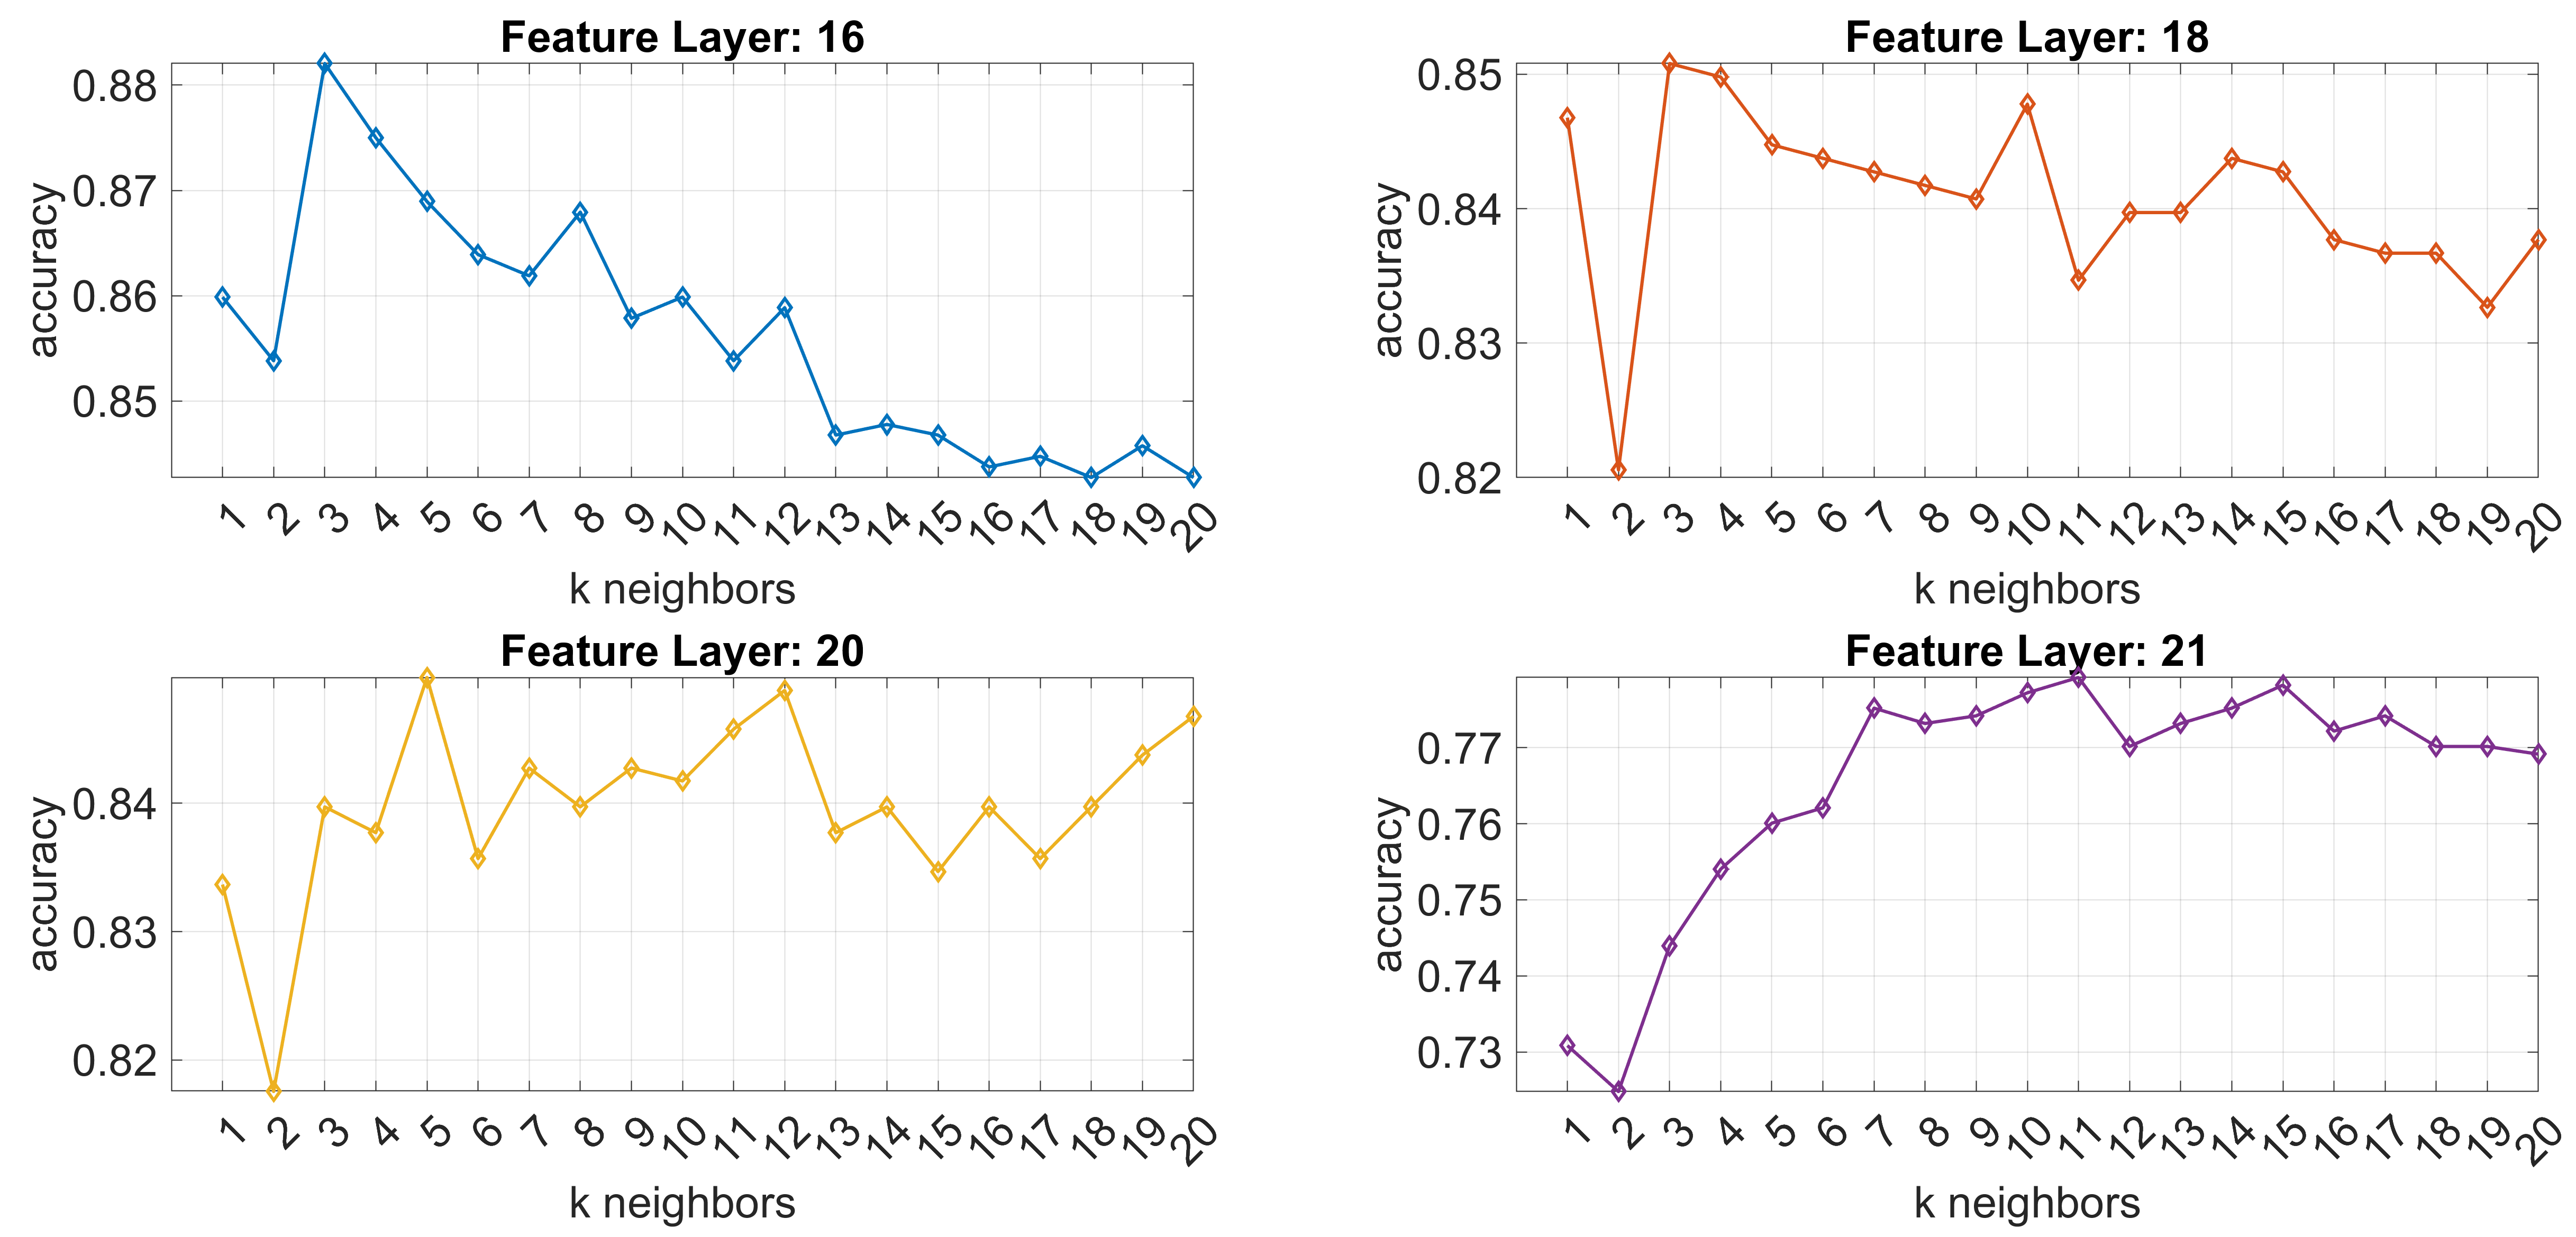
\includegraphics[width=.9\textwidth]{figures/ex5_1.png}
		\caption{Performance of KNN classifier for each feature (layer) by varing $k$ from $1$ to $20$.}
		\label{figknn}
	\end{figure}
	By choosing the best KNN classifier for each layer, a further comparison is given in Figure~\ref{figknn2}.
	\begin{figure}[ht]
	\centering
	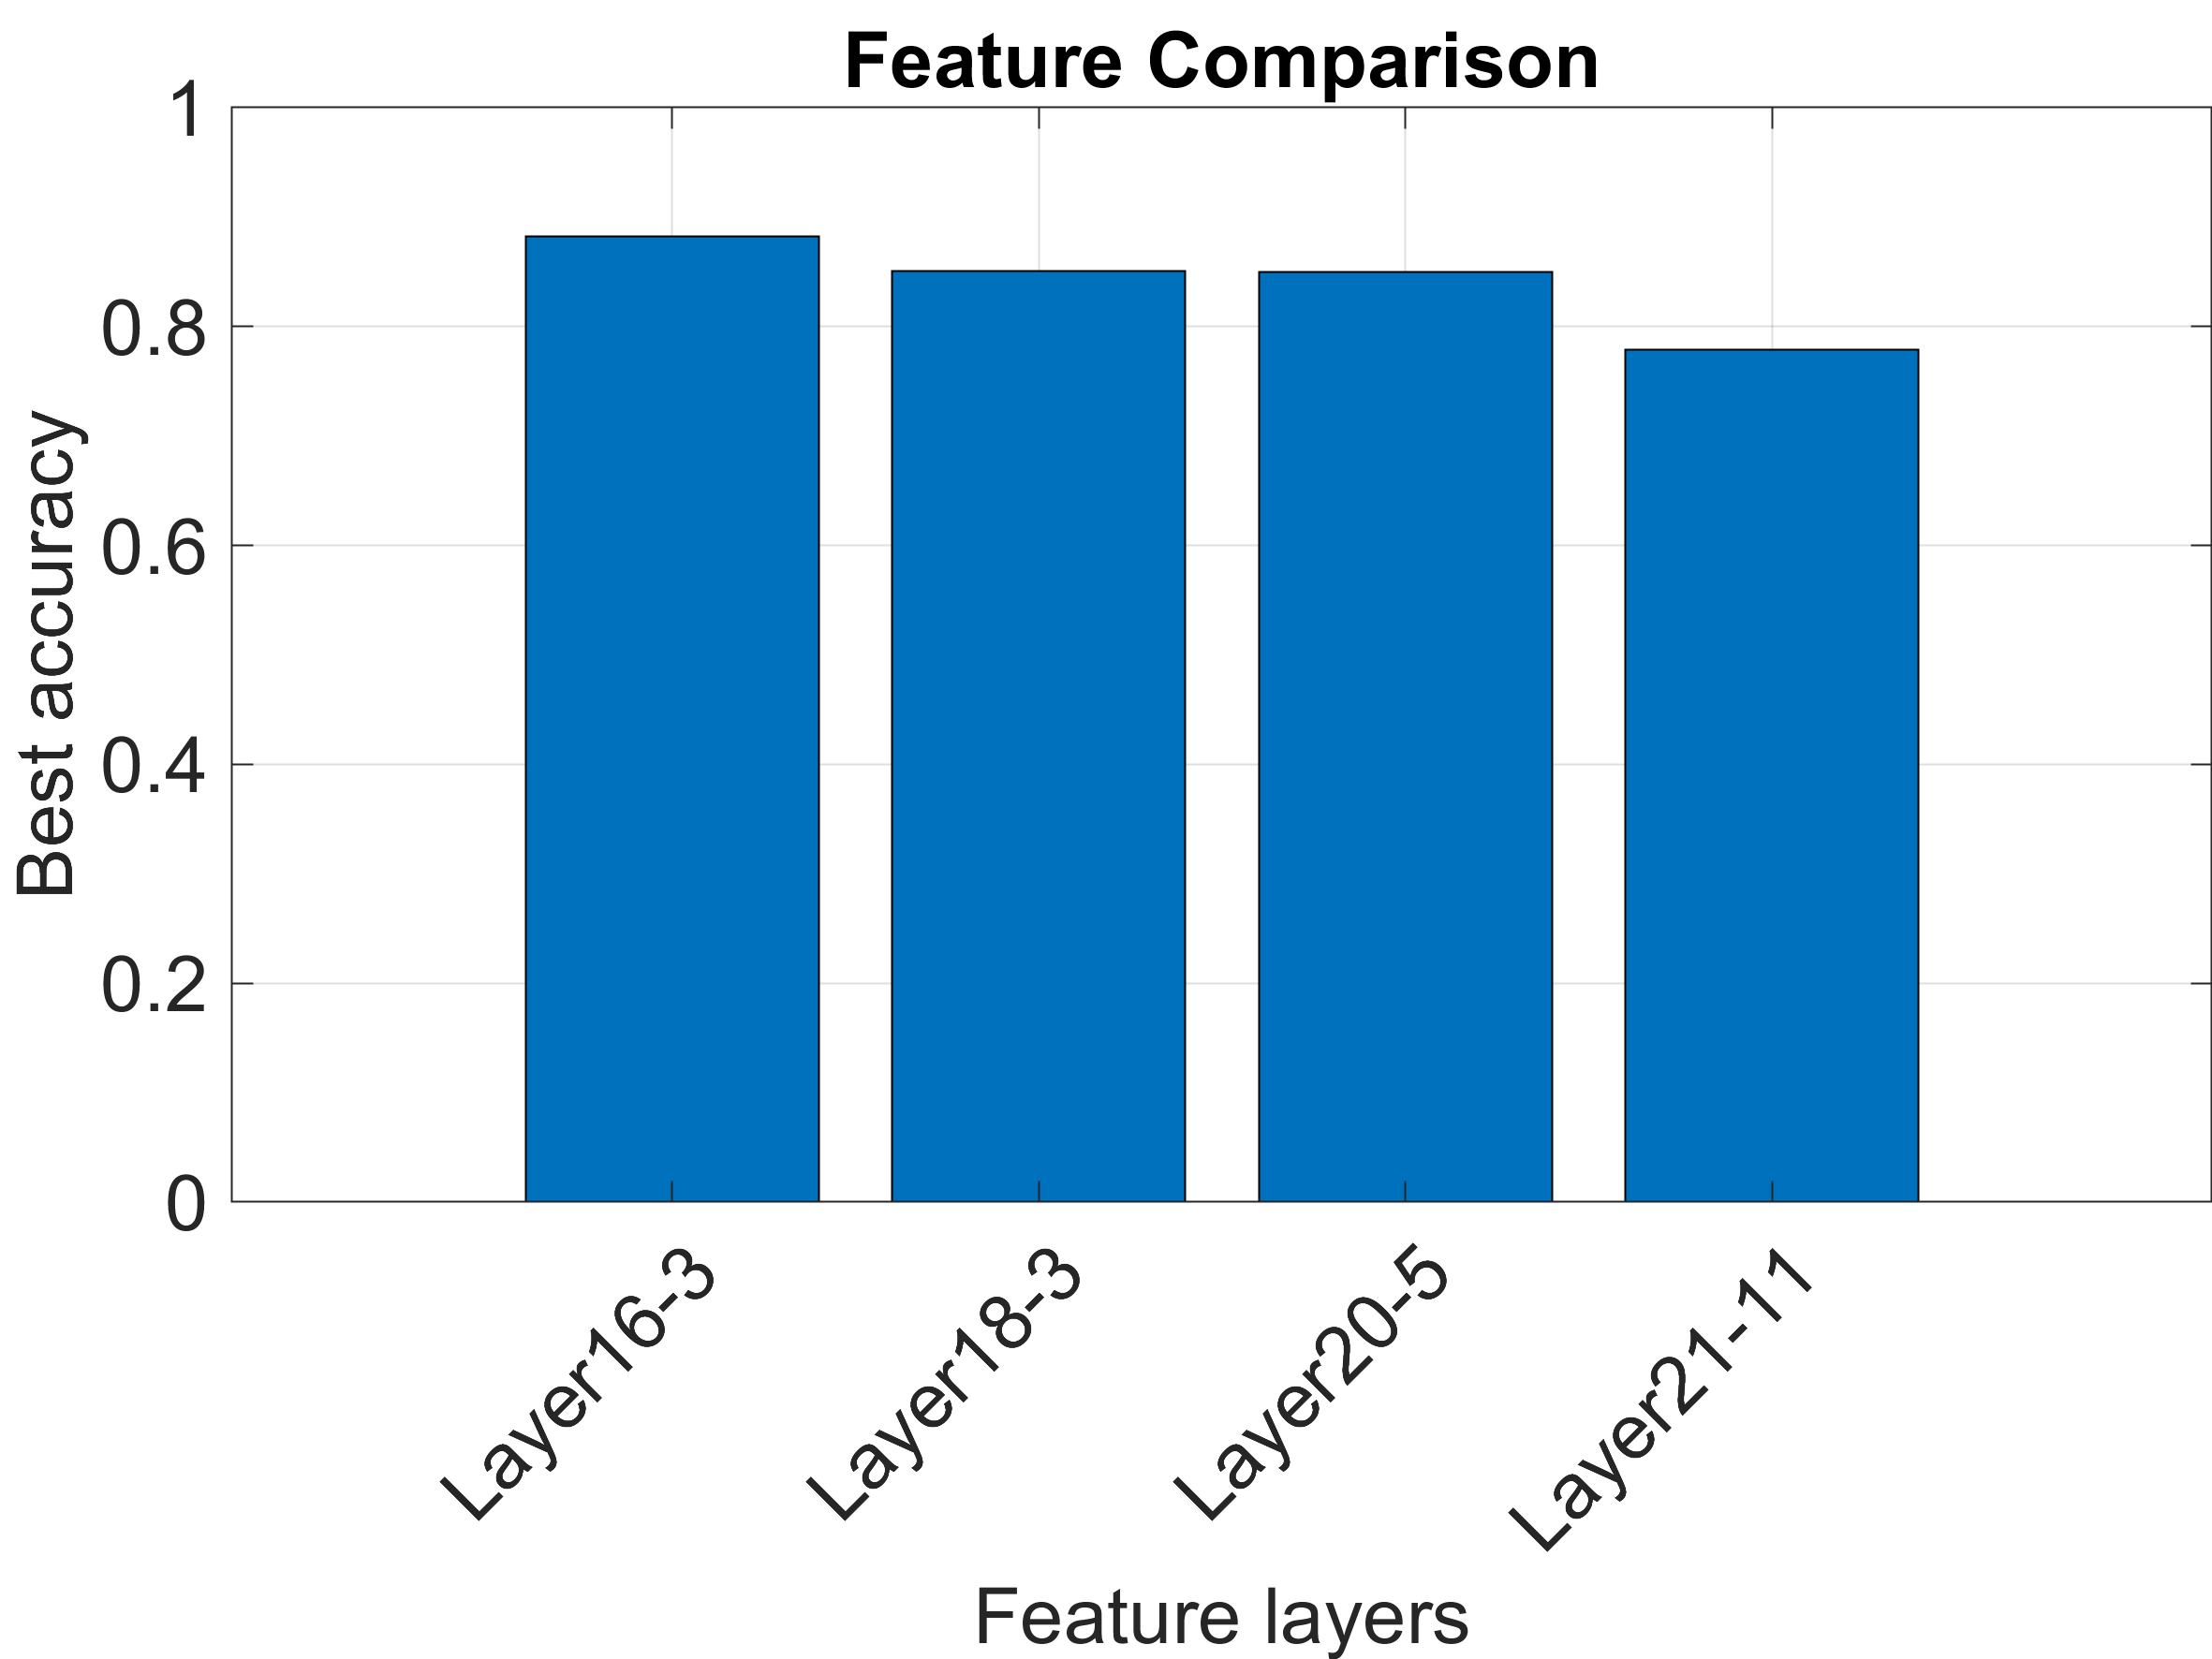
\includegraphics[width=0.5\textwidth]{figures/ex5_2.png}
	\caption{Comparion of the best KNN classifiers for each feature (layer). Clearly, choosing features from layer $16$ and setting $k=3$ will give the best result ($88.21\%$).}
	\label{figknn2}
\end{figure}
A further investigation is done by retraining the last $6$ layers of VGG19 using the CAMELYON17 dataset. The result is shown in Figure~\ref{figknn3}.
	\begin{figure}[ht]
	\centering
	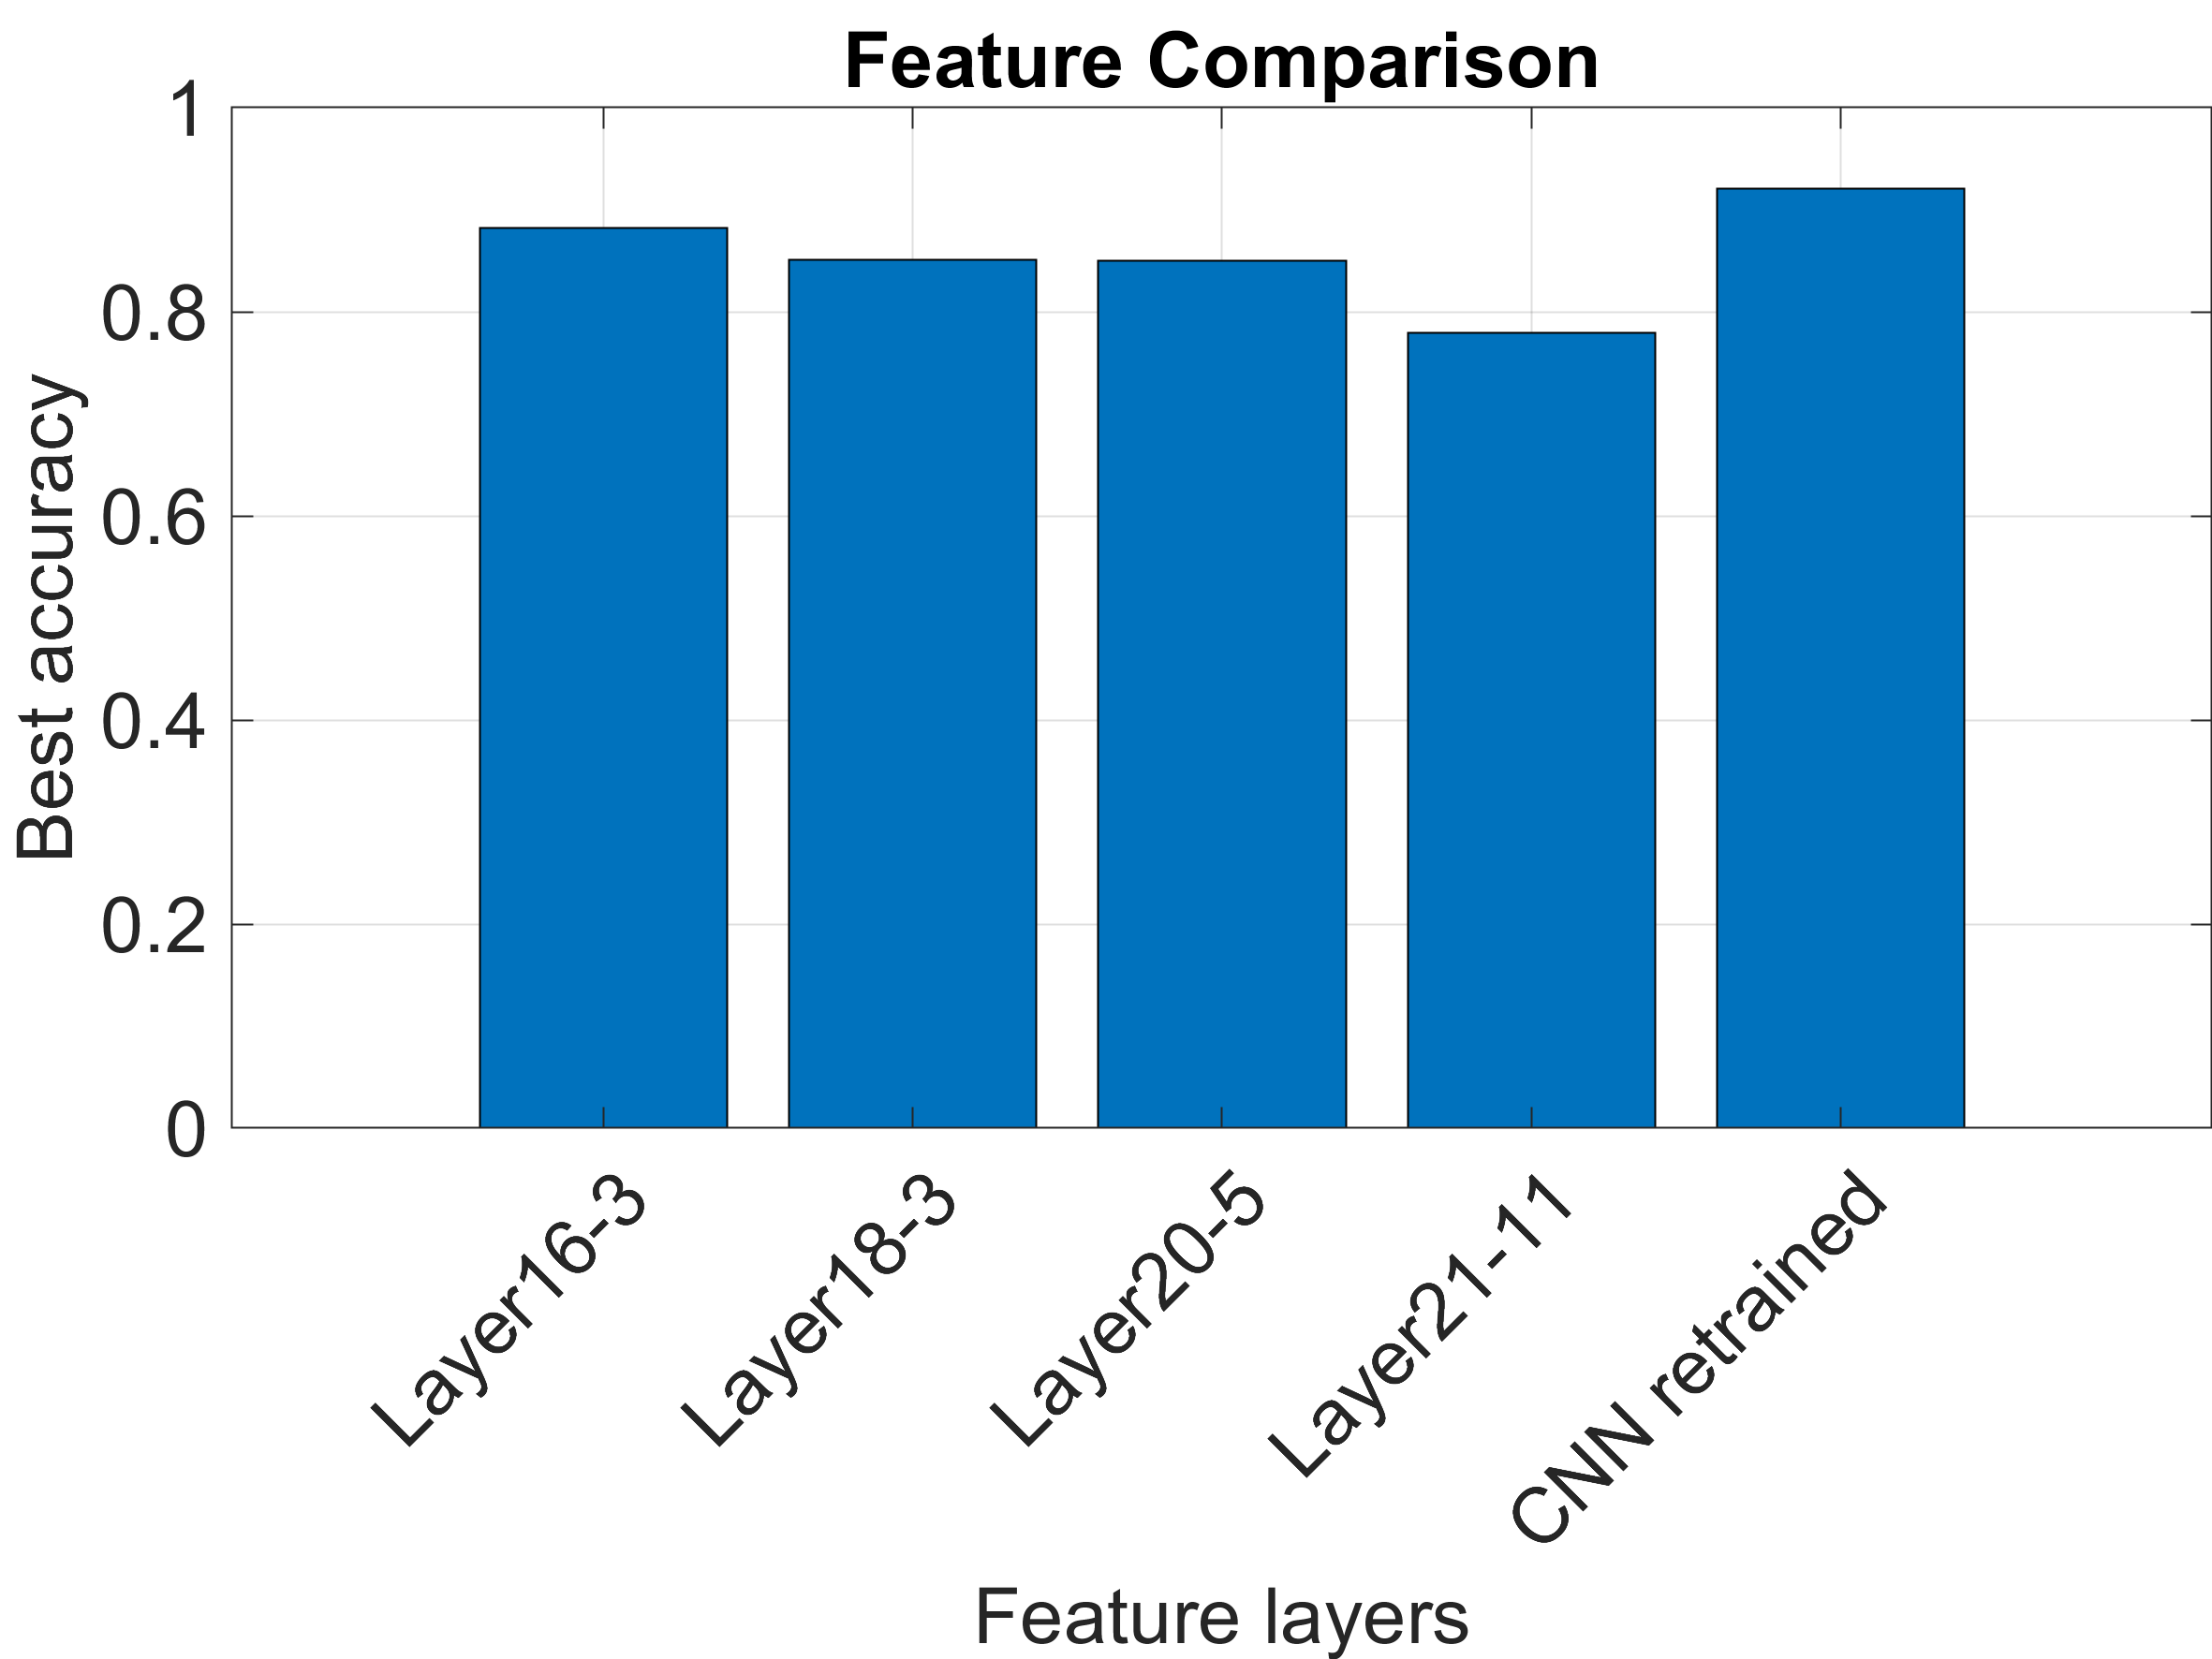
\includegraphics[width=0.5\textwidth]{figures/ex5_3.png}
	\caption{Comparion of the best KNN classifiers for each feature (layer) and retrained CNN. Clearly, retrained CNN shows the best result ($92.04\%$). However, it could be tricky since CNN is retrained using the same dataset, so for sure the retrained CNN will show very good result. The real performance needs to be checked with more data.}
	\label{figknn3}
\end{figure}

\section{MNIST}
For this I used a feed forward neural network with two layers:
\begin{itemize}
	\item First layer: inputs $784$ $+$ $1$ bias fully connected to $1000$ hidden neurons.
	\item Second layer: $1000$ hidden neurons $+$ $1$ bias fully connected to $10$ output neurons.
	\item Perform softmax to get the probability of each category.
\end{itemize}

The following strategies have been implemented and tried:
\begin{itemize}
	\item \textbf{SGD+Momentum:  faster convergence.}
	\item Adam:  faster convergence but showed no improvement on the final accuracy.
	\item \textbf{Minibatch: more stable gradient.}
	\item \textbf{Initialization from uniform distribution V.S. Gaussian distribution: initialization from uniform distribution showed better performance.}
	\item Weight decay or L$_2$ regularization: no improvement on the final accuracy.
	\item \textbf{Early stopping: helpful for avoiding overfitting.}
	\item \textbf{Data augmentation: random rotation $[-20^{\cdot},+20^{\cdot}]$, random translation $[-3,+3]$, random scaling $[0.8,1.1]$, random shearing $[-30^{\cdot},+30^{\cdot}]$, random image morphing (dilate or erode depends on a toss). Data augmentation is helpful with around 0.5\% improvement of the accuracy.}
\end{itemize}

The best net was trained with the following options:
\begin{itemize}
	\item  Optimization: SGD (0.01) +Momentum (0.9).
	\item Minibatch: 100.
	\item Initialization from uniform distribution.
	\item Early stopping: tolerance is 10.
	\item Data augmentation.
\end{itemize}
The best net can achieve an accuracy of \textbf{98.85\%}. Training is performed on a MacBook Pro with 2.6 GHz Intel Core i5 and 8 GB 1600 MHz DDR3 as the RAM. GPU was not used. Training could be finished within 10-30 minutes depending on the learning rate.

The final misclassified images are shown in Figure~\ref{figknn4}.
	\begin{figure}[ht]
	\centering
	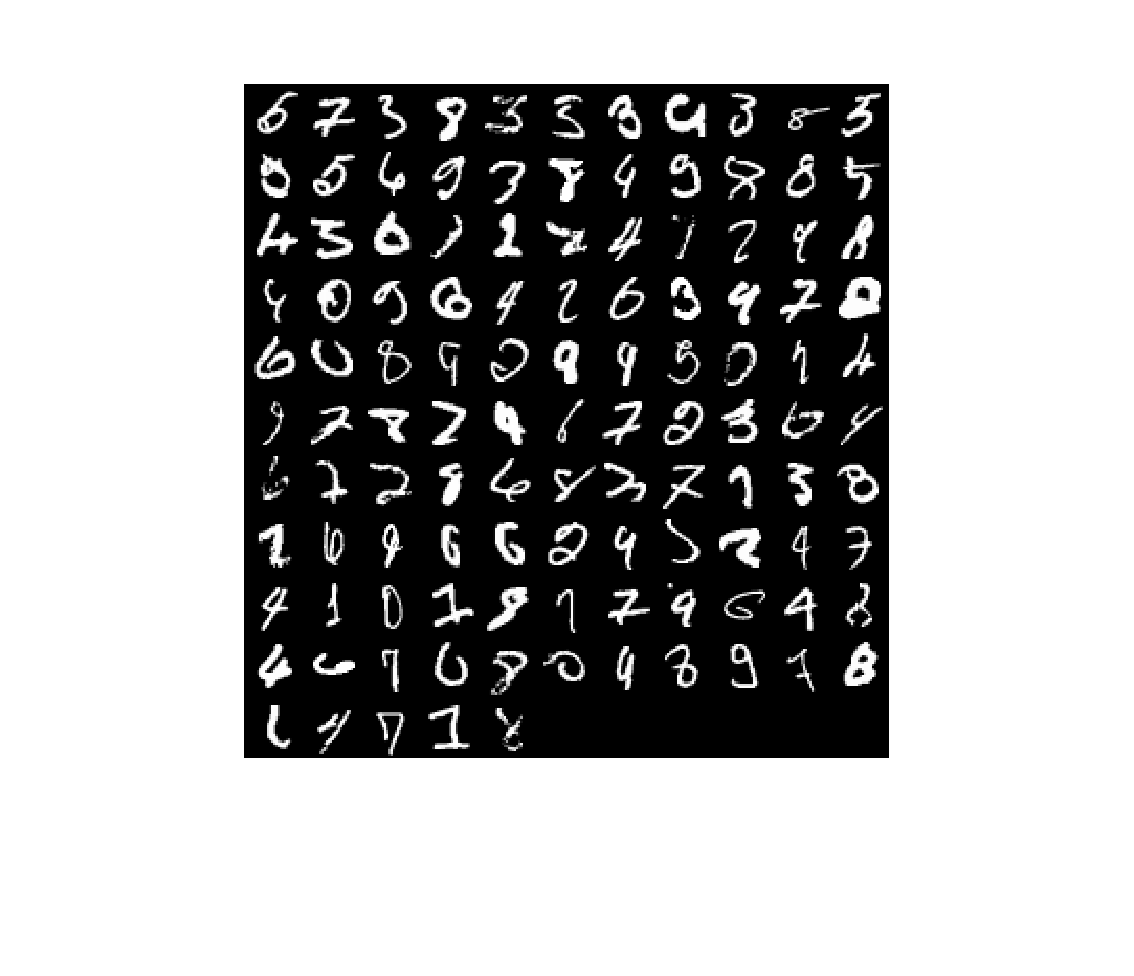
\includegraphics[width=1\textwidth]{figures/mnist1.png}
	\caption{Misclassified images.}
	\label{figknn4}
\end{figure}

%	\begin{figure}[htbp]
%	\centering
%	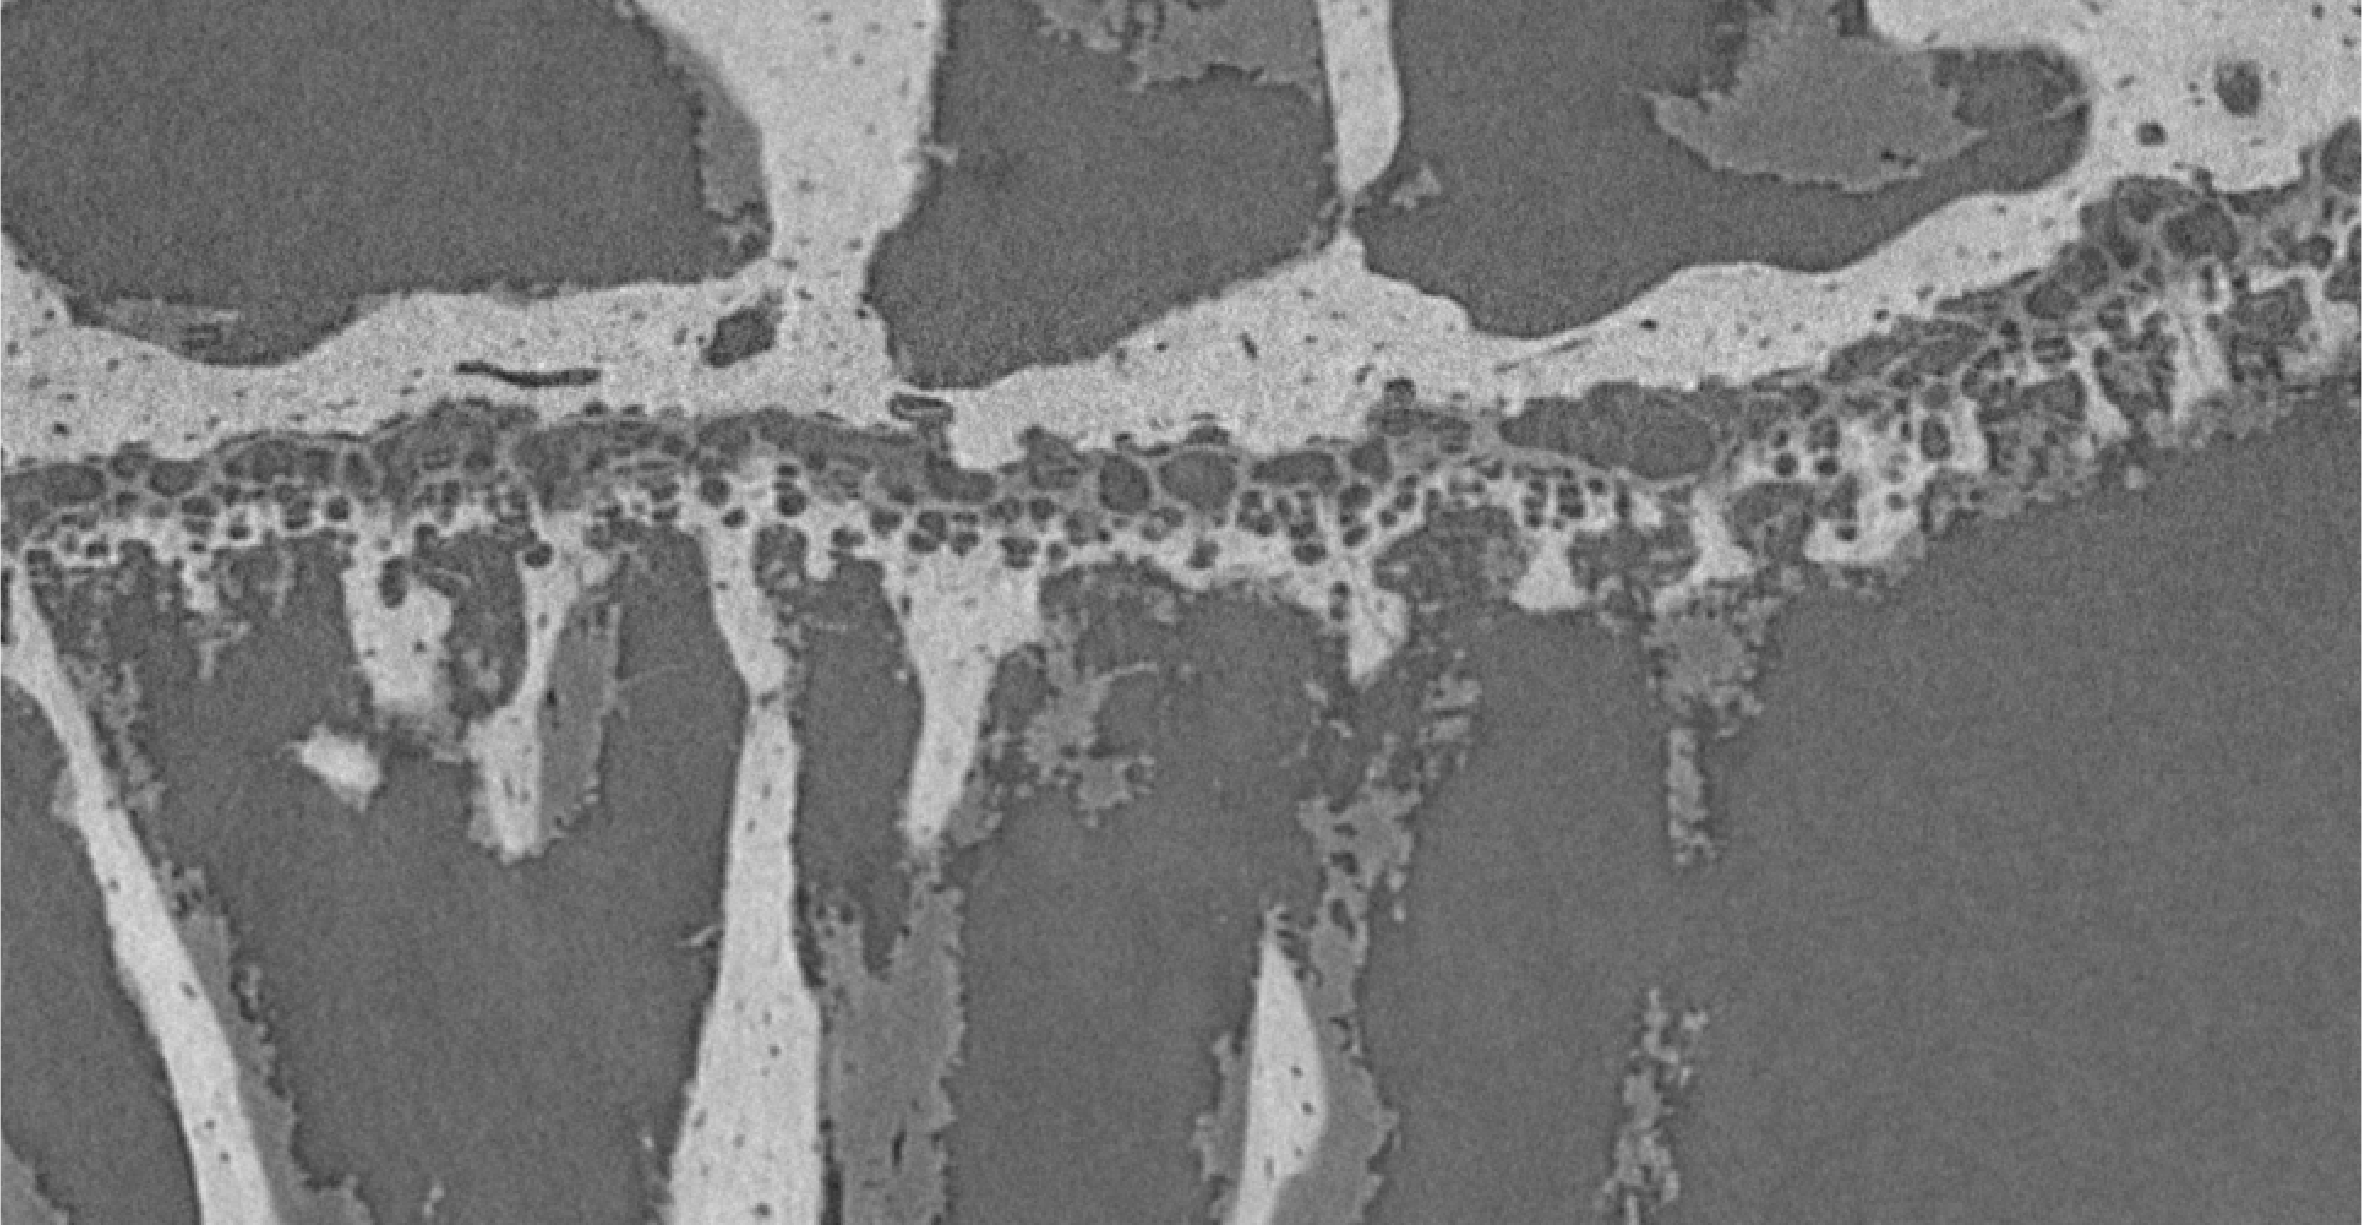
\includegraphics[width=0.5\textwidth]{./figures/assign2_raw.png}
%	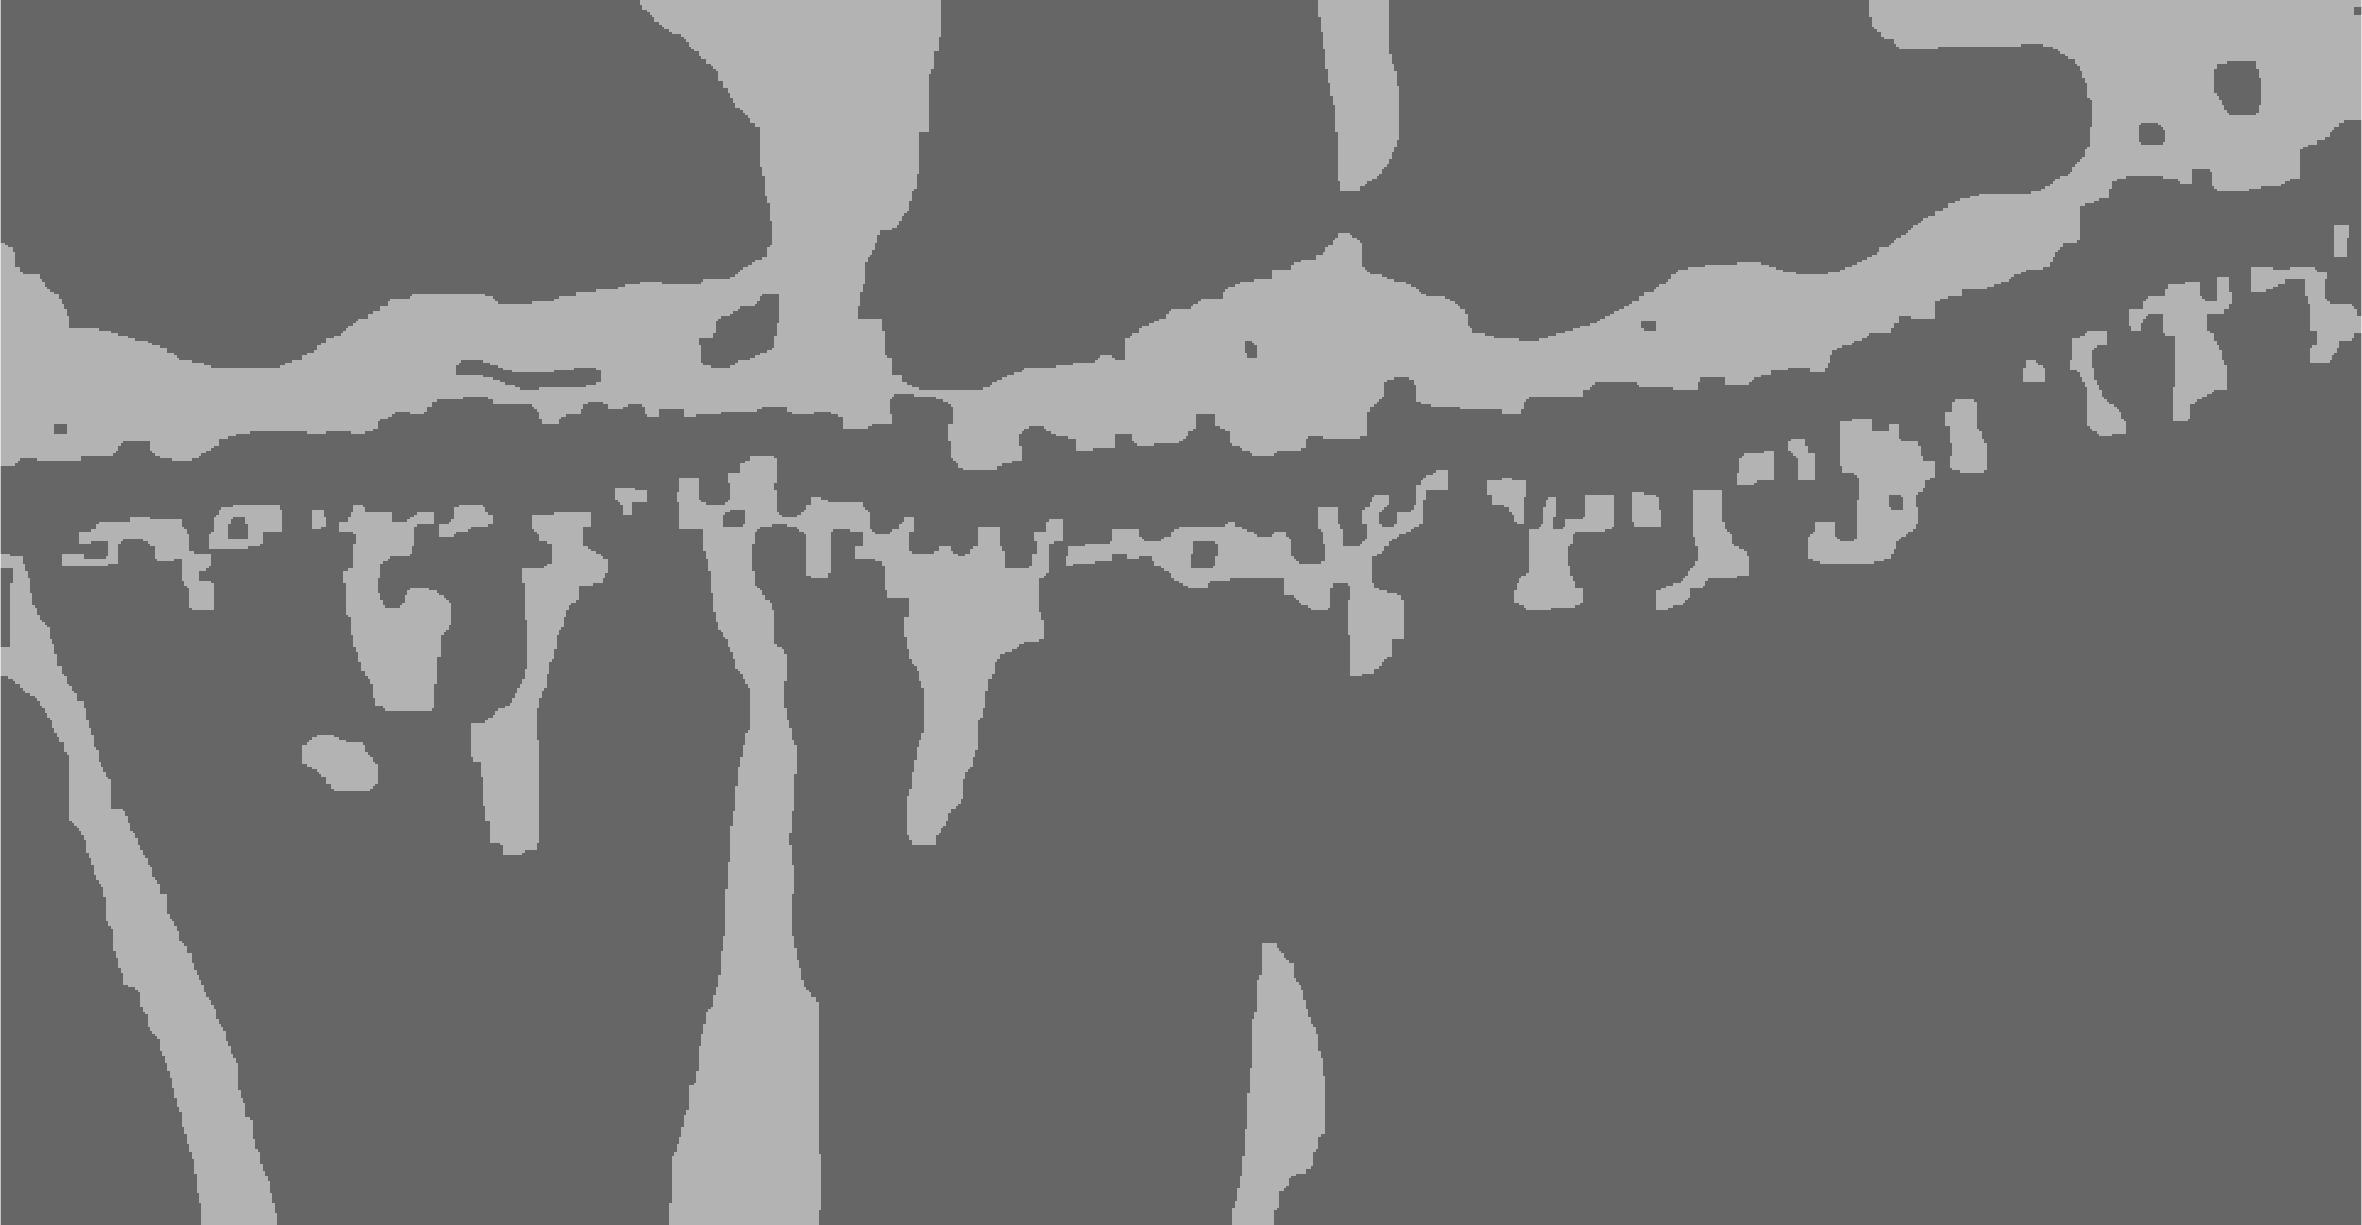
\includegraphics[width=0.5\textwidth]{./figures/assign2_seg.png}
%	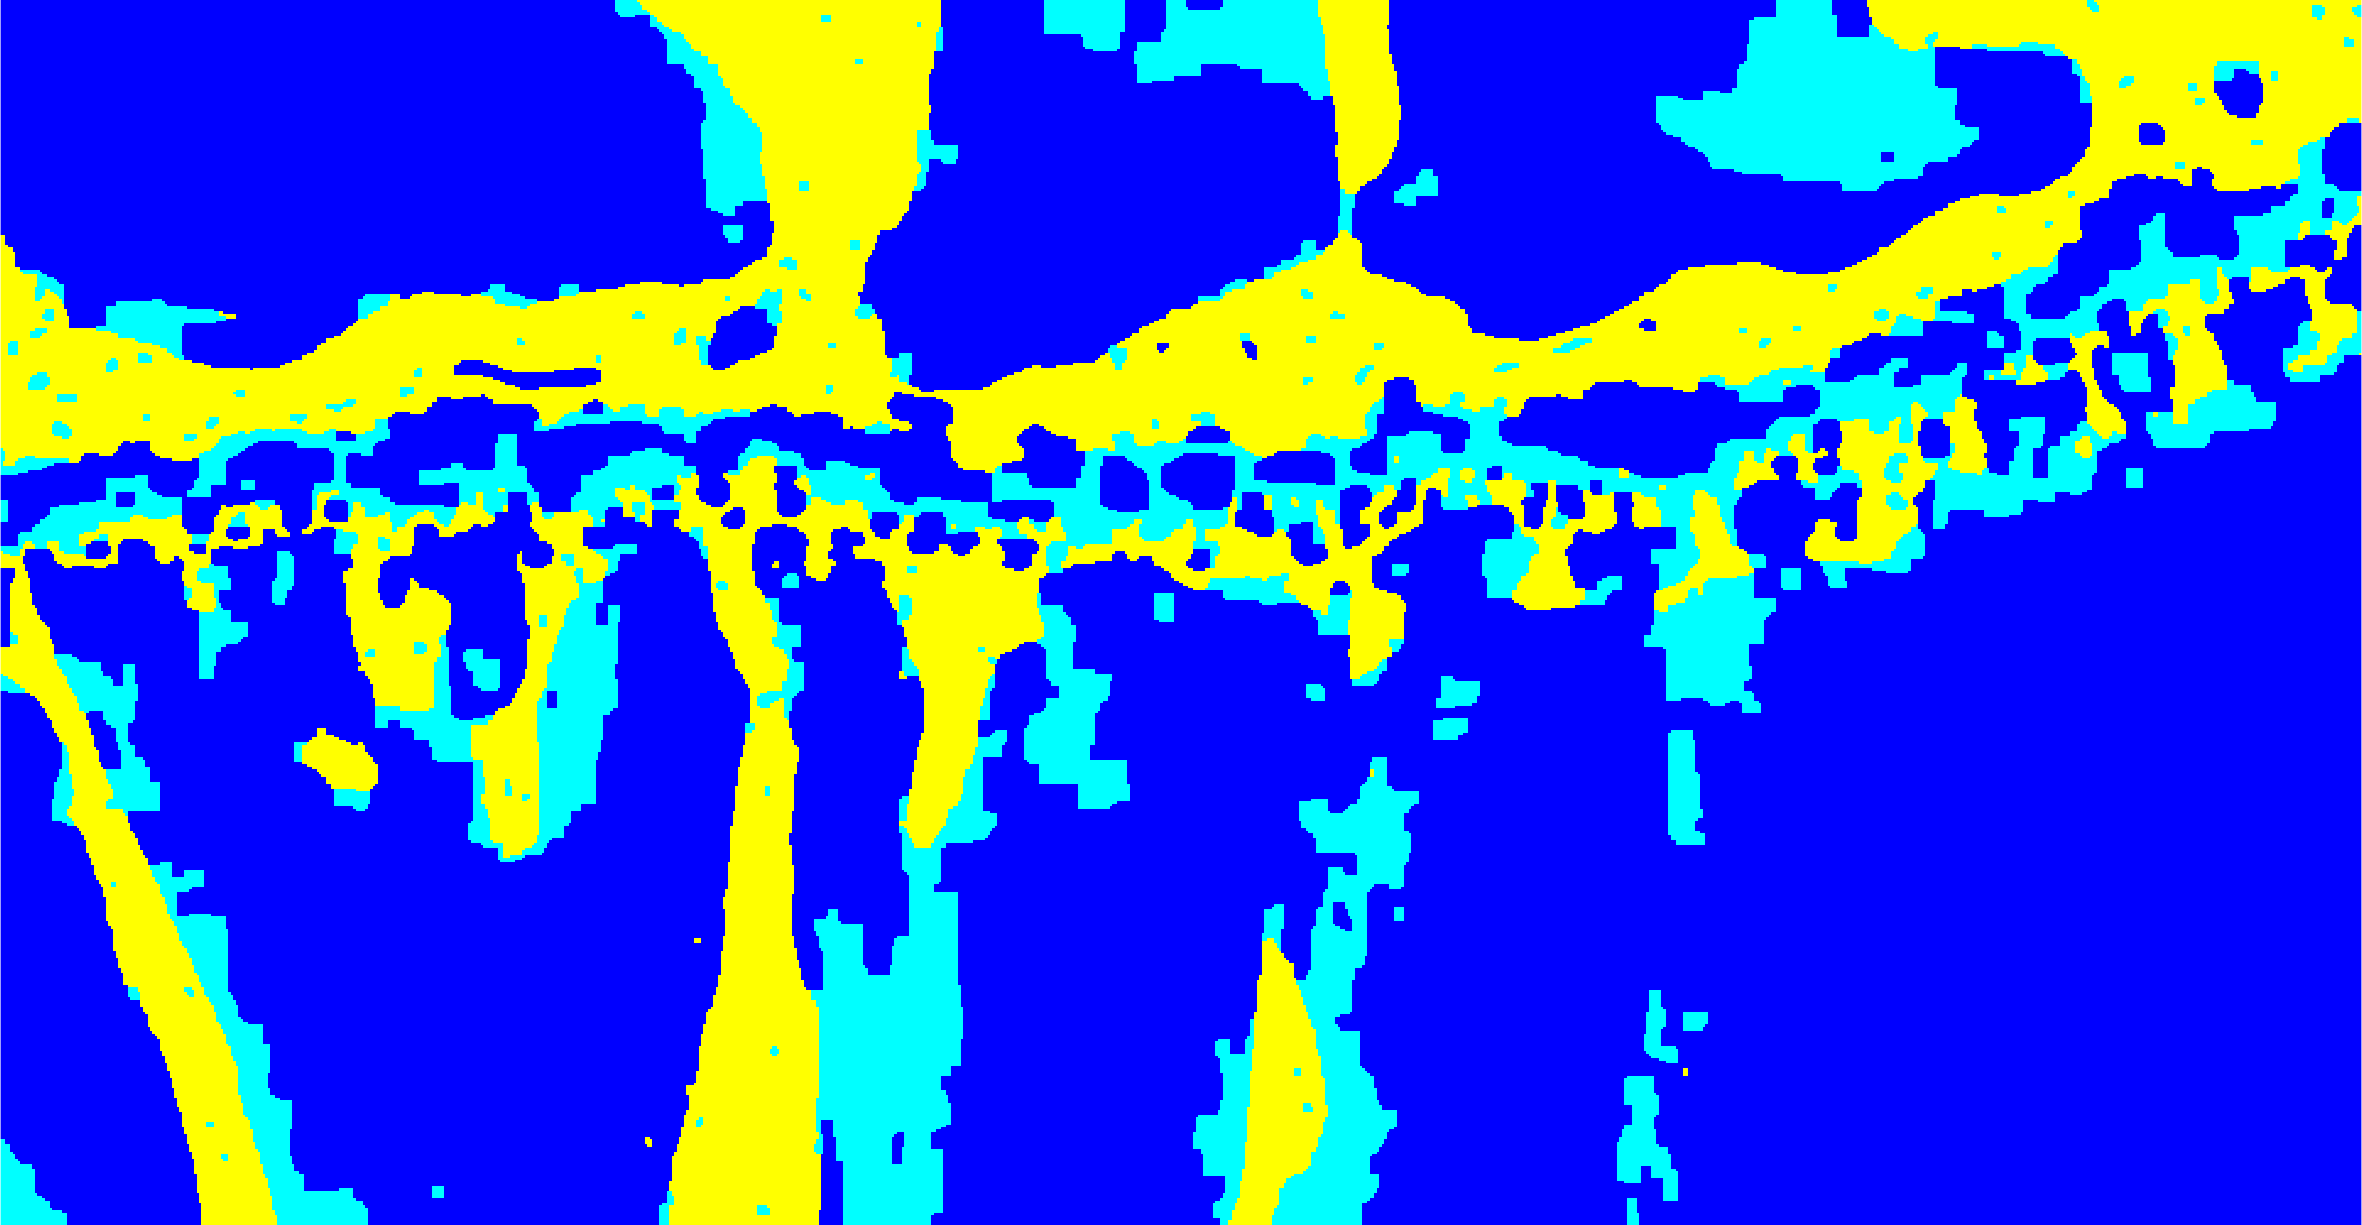
\includegraphics[width=0.5\textwidth]{./figures/assign2_mseg.png}
%    \caption{Middle image shows the segmentation of bone (bright) and air (dark). The bottom image shows the segmentation of bone (yellow), cartilage (light blue), and air (dark blue).}
%\end{figure}


	
%https://youtu.be/KMWywGcNNjI	
%https://youtu.be/_GslxUDEZzM
	
	%\bibliography{PnPCites} 
	%\bibliographystyle{ieeetr}
	
\end{document}